\documentclass[12pt]{tuthesis}
\def\dsp{\def\baselinestretch{2.0}\large\normalsize}

\usepackage{amsmath}
\usepackage{pgf}
%\usepackage{ifthen}
%\usepackage[framed,numbered,autolinebreaks,useliterate]{mcode} % Used for Matlab Code in Appendix
%\usepackage{breqn} % use dmath to help find manual breaks. 
%\usepackage{amsthm}
%\usepackage{amscd}
%\usepackage{graphicx}
%\usepackage{lscape}

\newtheorem{rem}{Remark}[chapter]
\newtheorem{alg}{Algorithm}[chapter]

\setlength{\oddsidemargin}{.75in}
\setlength{\evensidemargin}{.75in}
\setlength{\textwidth}{5.5in}


% Figure Scale Factors
% Chapter 1
    \pgfmathsetmacro{\ScaleModelImage}{0.75}
% Chapter 2
    \pgfmathsetmacro{\ScalePIDControlImageA}{0.85}
    \pgfmathsetmacro{\ScalePIDControlImageB}{0.95}
% Chapter 3
    \pgfmathsetmacro{\ScaleMLFigSteam}{1}
    \pgfmathsetmacro{\ScaleABFigThree}{0.75}
    \pgfmathsetmacro{\ScaleMLFigThree}{1}
% Chapter 4
    \pgfmathsetmacro{\ScaleMLFigFour}{0.75}

\begin{document}
    %% Declarations for Front Matter
    \title{A Comparison of Control Methods used on the Water Side of a Drum Boiler}
    \author{Robert A. Borzellieri, P.E.}
    \degreeyear{July, 2019}
    \degree{Master of Science in Electrical Engineering}
    \chair{Dr Saroj K. Biswas}
    \field{Electrical Engineering}
    \campus{}
    \maketitle
    \begin{frontmatter}
        \copyrightpage
        \begin{abstract}

This paper compares control strategies for a drum boiler unit. Drum Boilers are a highly nonlinear system, as there are non-minimum phase shrink-and-swell effects to account for. A more complex control strategy may prove to be a better option than what is used in industry today. The goal is to prove that Model Predictive Control (MPC) will provide superior results when compared to more classical approaches, like three element cascade control with a feed forward or using a Linear Quadratic Regulator (LQR).  

The process is built around the \r{A}str\"{o}m-Bell non-linear complex drum-boiler model. The model is extended with super-heater and turbine dynamics using an approach from an Iacob paper. The simplification of controlling heat flux directly will be used, instead of modeling the heat transfer and fuel combustion from the air side of the boiler. The implementation is carried out in MatLab. The simulation results are focused on automatic control operation and finding satisfactory response behaviors in each controller type. 

The simulated responses will be compared by a few defining characteristics, such as settling time, percent overshoot, and control energy used. 

\end{abstract}
        % \begin{acknowledgements}
% I want to thank my sister, for her support in helping me proofread this document, Dr Mihai Iacob for helping me understand his prior work, and Dr Saroj Biswas for his work as my advisor and teacher. 
% I would also like to thank my girlfriend and mother, both of whom have shaped me to be who I am today. 
% \end{acknowledgements}
        % \begin{dedication}\Large
% Grammarley 
%
% alyssaborzellieri@gmail.com
%
% Cookies05!
% \end{dedication}
        \tableofcontents
        \listoffigures
        \listoftables
    \end{frontmatter}
    
    % Start of Actual Document
    \chapter{Introduction}
\section{Overview of Steam Drum Control}

Industrial Boiler systems are used for many purposes, from supplying steam to various locations like hospitals to propulsion systems to the more common power generation. Boilers are now operating at higher pressure and are being built smaller than they were, and causes faster process control responses \cite{controlguruWebsite}. Because of high pressure operation, boilers must have an adequate level of control to stay safe. Due to the phenomena of minimum phase behavior and the shrink and swell effect, the boiler drum level control initially reacts in direct opposition to what is required for process stability. Shrink and swell refers to a phenomenon that when the drum pressure drops, some water in the tubes flashes, and those steam bubbles push water in the tubes above them up into the drum, temporarily raising the drum level. Then when the system stabilizes and those steam bubbles either collapse or reach the drum, the tubes rapidly refill with water from the drum, dropping its level. The effect is asymmetrical - when drum pressure rises due to falling steam demand, it temporarily suppresses the production of steam in the tubes but the effect is more subtle. \cite{crossco} This effect must then be accounted for if the system is to be properly controlled.  A Drum Boiler Schematic can be seen in Figure \ref{fig:schematic}.

% When the drum pressure drops, some water down in the tubes flashes, and those steam bubbles push water in the tubes above them up into the drum, raising the drum level even as the total mass of water in the drum and tubes falls.

\begin{figure}[ht]
    \begin{center}
    \resizebox{\ScaleModelImage \textwidth}{!}{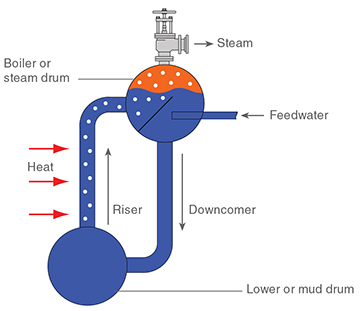
\includegraphics{Graphics/Graphic.png}}
    \caption{Drum Boiler Schematic \cite{spiraxsarcoWebsite}}
    \label{fig:schematic}
    \end{center}
\end{figure}

\section{Literature Review}


Mathematical models for a Boiler-Tubine system exist in the literature, however most are simplified to not include the dynamics of the drum's water level nor the shrink and swell effect. The model developed by \r{A}str\"{o}m and Bell \cite{Astrom} provides sufficient detail to model these parameters.
An extension of this model was developed by Iacob and Andreescu \cite{Iacob} which provides modeling for the feed-water valve, fuel flow valve, steam valve, throttle pressure, and power output. 

Steam boiler is a highly nonlinear system which poses significant complexities in its control system design and analysis.  Conventional control method is known as {\it three element control} in the industry, which is effectively a PID type control system that regulates three measured quantities in the boiler, such as liquid level in the drum, feed water flow, and steam flow leaving the drum.  The three-element control is based on linearized dynamics of the boiler that provides the required boiler performance when the deviation of the state variables remains relatively small with respect to the nominal state.  This research investigates design of boiler control system that is expected to provide a better system performance when large variations of the system state may occur.



\section{Goals and Objectives of proposed research}

%%% Section 1.3 needs some narrative rather than bullet points.  Typically the outline should be
%%% a) the goals of the research
%%% b) scope of the research/methodology

The broad objective of this research is to develop a control system that provides the desired performance of the steam boiler for a wider range of its operating state.  Conventional three-element control or other linear control methods which rely on linearized model of the boiler have limited performance as the boiler must operate near the nominal operating point of the system.  This research explores the application of the Model Predictive Control (MPC) for the design of the boiler control system.  In recent years, MPC control method has found significant attention in industry \cite{Wang, Forbes, Zang, Botelho} and academia \cite{Saltık, Ghosh, Song} alike with excellent performance.  There are several advantages of the MPC control system that make it an ideal candidate for its application to the boiler control, such as 1) it does not require that the system operate near a nominal operating point, 2) it is easy to include various constraints in the control design, and 3) it is possible to design a controller even when the system model is not precisely known.

The goals of this thesis are

\begin{itemize}
  \item Review mathematical model of the steam boiler
  \item Investigate limitations of conventional control systems, such as PID and LQR
  \item Apply model predictive control system to the steam boiler and analyze its performance
\end{itemize}

The developed control system will be evaluated by simulation only as there are no experimental facilities are available.  For the mathematical model of the boiler, we will consider the \r{A}str\"{o}m and Bell \cite{Astrom} model which is quite well known in the literature.  The closed loop system will be analyzed in Matlab/Simulink environment under various operating conditions. 

\section{Outline of the Thesis}

This following is an outline of the rest of this thesis proposal: Chapter 2 presents the basics of the three-element control and the LQR control which will be followed by details of Model Predictive Control design method.  In Chapter 3 we present the \r{A}str\"{o}m and Bell \cite{Astrom} model of the steam boiler and the model validation.  Chapter 4 presents some simulation results of three-element control and the LQR control.  Chapter 5 outlines plans for further research on application of MPC control and conclusions. 



    \chapter{Control Methods for Nonlinear Systems}
    The boiler system is inherently nonlinear so that an adequate control method must be implemented for its safe and efficient operation.
    Common industry practice in this respect is to implement the three-element control, which is fundamentally the PID control structure which is first discussed. Then we also present the linear quadratic control (LRQ) which is a powerful control method used in many industrial applications, which however has its limitations when applied to nonlinear systems. In fact, both PID and LQR control methods cannot be used for nonlinear systems unless the system model is linearized. As is well known, the linearized model is valid only if the process operates in a small neighborhood with respect to the nominal operating state. For large variations in the operating state, it is necessary that a nonlinear control method be utilized. The Model Predictive Control (MPC) is one of the powerful, yet simple, methods for controlling nonlinear systems, and has attracted the attention of engineers in the profession. This chapter introduces the fundamentals of the MPC control method, which will be used in this thesis for controlling the steam boiler.

    \section{Three Element Level Control}
        Three Element Control refers to the number of measurements or Process Variables (PV) that are used in the control calculation. These measured elements are:
        
        \begin{itemize}
          \item $l$ - Liquid Level in the Drum
          \item $q_f$ - Feed-water Flow into the Drum
          \item $q_s$ - Steam Flow leaving the Drum 
        \end{itemize}
        
        \begin{figure}[ht]
            \begin{center}
                \resizebox{\ScalePIDControlImageA \textwidth}{!}{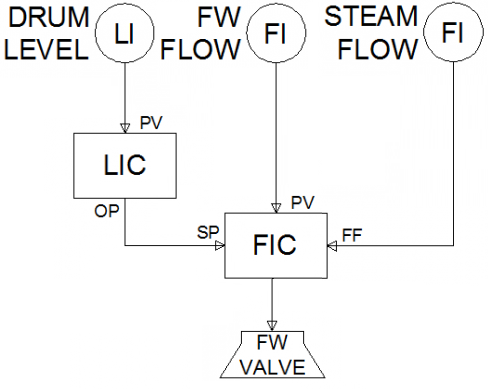
\includegraphics{Graphics/Three_Element}}
                \caption{Three Element Control \cite{crossco}}
                \label{fig:3_element_control}
            \end{center}
        \end{figure} 
        
        Three Element Control \cite{crossco} consists of two PI(D) loops in cascade control, and a feed forward control. This can be seen in Figure \ref{fig:3_element_control}. The two loops in cascade are a fast acting internal loop for feed-water and a slower external loop for drum level. In a cascade control scenario, the external loop's output (OP) is used as the Set Point (SP) for the inner loop. 
        The feed forward (FF) of steam flow is applied to the internal loop. An alternative, and less popular configuration can have the feed forward on the outer loop, as seen in Figure \ref{fig:Alt_3_element_control}. It should be noted that a cascaded control setup has several drawbacks, including integral windup due to the inner loop being at a physical limit but the outer loop still attempting to control. 
        %{\bf Give a better description of the two figures on three element control.  There are many symbols that are not defined.} % Biswas Notes % % Robs Notes - Should be fixed in above paragraph %

        \begin{figure}[ht]
            \begin{center}
                \resizebox{\ScalePIDControlImageB \textwidth}{!}{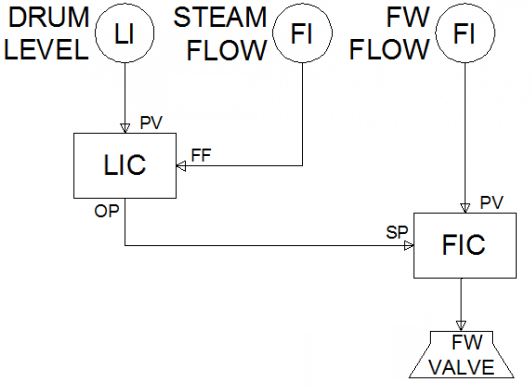
\includegraphics{Graphics/Three_Element_2}}
                \caption{Alternative Three Element Control \cite{crossco}}
                \label{fig:Alt_3_element_control}
            \end{center}
        \end{figure}



        %{\bf Add a paragraph on {\it shrink and swell} effect here}.   %% BISWAS NOTES %%
        %Shrink and swell refers to a phenomenon that when the drum pressure drops, some water in the tubes flashes, and those steam bubbles push water in the tubes above them up into the drum, temporarily raising the drum level. Then when the system stabilizes and those steam bubbles either collapse or reach the drum, the tubes rapidly refill with water from the drum, dropping its level. The effect is asymmetrical - when drum pressure rises due to falling steam demand, it temporarily suppresses the production of steam in the tubes but the effect is more subtle. \cite{crossco} 
        % Rob Notes - Moved to chapter 1 %
        
        Single Element and Two Element control are used at lower feed-water flows or lower load, where the shrink and swell effects are not as prevalent. Single Element control is a PI(D) Level control loop, and Two Element control is the same as Three Element control, without the feed forward.
        
        %The cascade control must be tuned with the following procedure. The outer loop is switched to manual mode and the inner loop is tuned, then, the inner loop is placed in automatic control mode and the outer loop is tuned.
        
        In this control mode, Throttle Pressure is usually controlled by a simple PI(D) loop. Total power output may be controlled instead of throttle pressure. The turbine is often modeled as a first order system with the input of Throttle Pressure and the output of mechanical power \cite{controlguruWebsite}.

        \subsection{Application in Boiler Controls}

        By design, the PID control is used to minimize error with respect to a desired operating reference using specific tuning parameters. It does not allow any optimization of the process operation, such as minimization of fuel consumption (or control energy), nor does it account for any boundary conditions. Industry experts also use adaptive tuning controllers due to the fact that the tuning parameters can vary with load. Optimization of process operation could be achieved using optimal  and robust control methods as presented next.

    \section{Linear Quadratic Regulator}
    
        The Linear Quadratic Regulator (LQR) is one of powerful methods for optimizing the process operation.  In this method, the system performance is defined in terms of a cost function which is a measure of cost of state error and cost of control.  The objective is to find a control that minimizes the cost function.  For a discrete time linear system,
        
        \begin{equation} 
            \label{eq:lqr1}
            x(k+1) = A x(k) + B u(k)
        \end{equation}
        
        where $x_k$ is the state vector and $u_k$ is the control vector, and the state and control matrices $A$ and $B$ are of compatible dimension.  The cost function is taken as
        
        \begin{equation}
            \label{eq:lqr2}
            J = \sum_{0}^{\infty} \left ( x_k^T Q x_k + u_k^T R u_k\right )
        \end{equation}
        
        where $Q$ is a positive semidefinite matrix and $R$ is a positive definite matrix.
        Here the first term of the cost function represents the cost due to state error with respect to the reference (which is taken as zero in this case), and the cost of control.
        The optimal control sequence that minimizes the cost function is given by the discrete time Riccati equation
        
        \begin{equation}
            \label{eq:lqr3}
            \aligned
                P &= A^TPA - (A^TPB)(R+B^TPB)^{-1}(B^TPA)+Q\\
                K_{lqr} & = (R+B^TPB^{-1})(B^TPA)\\
                u_k & = K_{lqr} x_k
            \endaligned
        \end{equation}
        
        By solving the Riccati equation, one obtains the matrix $P$ which is a positive symmetric definite matrix, which is then used to find the feedback gain $K_{lqr}$ for the control loop.  In this method, the Riccati matrix $P$ can be computed before the control loop initiates.  From the design perspective, one must choose the appropriate weighting matrices $Q$ and $R$ matrices so as to obtain the desired closed loop performance.
        
        It is important to note that the linear quadratic regulator as discussed above applies to linear systems only.  However there are many practical systems, including the steam boiler discussed in the thesis, are described by nonlinear system model.  For nonlinear systems, one can linearize the system model and then apply the LQR theory.  However the drawback is that this approach works well only when the actual nonlinear system operates within a small neighborhood of the operating point.  For large variations of the system state, the results are usually not acceptable.
        
        %Linear Quadratic Regulators in both the Continuous and Discrete form are solved using different forms of the Riccati Equation. This is useful for Linear systems, as in the name of the control methodology itself describes the type of system it is used in. The Quadratic portion of the name refers to the cost function. Traditional LQR applications in a nonlinear system would see the system being linearized around a point, and providing designing the regulator around that point.
        
        There is some research in applying LQR methodologies to nonlinear systems using the State-Dependent Riccati Equation \cite{Korayem}.  In this method, the one derives  the Riccati equation in which the system model matrices is actually dependent on the current system state.  So fundamentally, this means that the Riccati equation must be solved in real time for each sampling time before the control input is computed. This is not a trivial job as it takes significant computing resources to solve the Riccati differential equations.
        
        % https://math.stackexchange.com/questions/2558102/lqr-controller-for-a-nonlinear-system-how-to-split-the-ss-model-as-a-and-b-mat
        % https://ac-els-cdn-com.libproxy.temple.edu/S0019057814001268/1-s2.0-S0019057814001268-main.pdf?_tid=fe049522-ada0-4187-ad8b-4411fe3bf75d&acdnat=1539568348_aa431eef8ff6d9743feeae876ede3752
        
    \section{Model Predictive Control}
    
        Model predictive control (MPC) \cite{Wang} is a popular control method that has found many applications in chemical industries. MPC is an advanced control method that optimizes the current state satisfying process constraints while at the same time using predicted information of system state in future time slots.
        MPC control strategies are characterized by a explicitly and separately identifiable model of the controlled system. This model is used to calculate the behavior of the plant with the future control signal as adjustable variables.
        
        MPC has direct links to the classical linear quadratic regulator (LQR) in continuous time and discrete time when using a long prediction horizon. The key difference between MPC and LQR is that the MPC solves the optimization problem using a moving time horizon window and optimized along the entire time horizon, while LQR solves the same problem within a fixed window and solves for a single optimal solution.
    
        \subsection{Discrete Time MPC Theory}

            The MPC control method is a receding horizon control method in which one first finds the optimal solution for a predicted time horizon, but apply the control for only one time step.  The process is then repeated for future time slots.
            Consider the linear system in discrete time
            \begin{equation}
                \label{eq:mpc1}
                \aligned 
                    x(k+1) & = A x(k) + B u(k)\\
                    y(k) & = C x(k)
                \endaligned
            \end{equation}
            Denote the control signals for the entire control horizon starting from time slot $k_i$ as
            \begin{equation}
                \label{eq:Trajectory1}
                U(k_i) = \{u(k_i), u(k_i+1), ... , u(k_i+N_c+1)\}
            \end{equation}
            where $N_c$ is the Control Horizon. Then future system States can be denoted as:
            
            \begin{equation}
                \label{eq:mpc2}
                \aligned
                    x(k_i+1|k_i)  =& Ax(k_i) + B u(k_i)\\
                    x(k_i+2|k_i)  =& Ax(k_i+1|k_i) + B u(k_i+1)\\
                                  =& A^{2}x(k_i) + AB u(k_i) + B u(k_i+1)\\
                    x(k_i+3|k_i)  =& Ax(k_i+2|k_i) + B u(k_2+1)\\
                                  =& A^{3}x(k_i) + A^2B u(k_i)+ AB u(k_i+1) + B u(k_i+2)\\
                    x(k_i+N_p|k_i)=& A^{N_p} x(k_i) + A^{N_{p}-1} B u(k_i+1-1) + \cdots\\
                                   & \cdots + A^{N_{p}-N_{c}} B u(k_i+N_c-1)
                \endaligned
            \end{equation}                

            where $N_p$ is the Prediction Horizon. 
            
            Using the above equation, future Controlled Outputs can be computed as:
            \begin{equation}
                \aligned
                    y(k_i)        =& Cx(k_i)\\
                    y(k_i+1|k_i)  =& CAx(k_i) + CB u(k_i)\\
                    y(k_i+2|k_i)  =& CA^{2}x(k_i) + CAB u(k_i) + CB  u(k_i+1)\\
                    y(k_i+3|k_i)  =& CA^{3}x(k_i) + CA^2B u(k_i)+ CAB u(k_i+1) + CB u(k_i+2)\\
                    y(k_i+N_p|k_i)=& CA^{N_p} x(k_i) + CA^{N_{p}-1} B u(k_i+1-1) + \cdots\\
                                   & \cdots + CA^{N_{p}-N_{c}} B u(k_i+N_c-1)
                \endaligned
                \label{eq:outputs1}
            \end{equation}   
            
            The control horizon $N_c$ is chosen to be less than (or equal to) the prediction horizon $N_p$.
            It should be noted that all predicted variables are calculated from the current state, future control movements, and the model information.
            The above equations then can be expressed in matrix form as:
            %{\bf why do you need a control horizon different from prediction horizon?}
            %% Notes Needed Here BISWAS BORZELLIERI %%
            
            \begin{equation}
                \label{eq:Matrix1}
                Y = Fx(k_i) + \Phi U(k_i)
            \end{equation}
            where
            \begin{equation}
                \aligned
                    Y &= \left [ \begin{array}{c} y(k_i+1|k_i) \\ y(k_i+2|k_i)\\\vdots \\ y(k_i+N_{p}|k_i) \end{array}  \right ], \\ \\
                    U &=\left [  \begin{array}{c} u(k_i) \\ u(k_i+1) \\\vdots \\ u(k_i+N_{c}-1) \end{array}  \right ]\\ \\
                    F &= \left [ \begin{array}{c}CA \\ CA^{2}\\\vdots \\ CA^{N_{p}} \end{array}  \right ]\\ \\
                    \Phi &= \left [ \begin{array}{ccccc}
                         CB & 0 & 0 & \cdots & 0 \\
                         CAB & CB & 0 & \cdots & 0 \\
                         CA^{2}B & CAB & CB & \cdots & 0 \\
                         \vdots & \vdots & \vdots & \ddots & \vdots \\
                         CA^{N_{p}-1}B & CA^{N_{p}-2}B & CA^{N_{p}-3}B & \cdots. &  CA^{N_{p}-N_{c}} B \end{array}  \right ]
                \endaligned
            \end{equation}
            
            Suppose the control objective is for the system output $y(k_i)$, $y(k_i+1)$, $\cdots$, $y(k_i+N_p)$ to follow a desired output. Define the set-point desired reference as
            \begin{equation}
                \label{eq:mpc5}
                \aligned
                    R_s &= \overline{R}_s r(k_i)\\
                    \overline R_s^T &= \overset{N_p}{\overbrace{\begin{bmatrix} 1& 1 & ... & 1 \end{bmatrix}}}
                \endaligned
            \end{equation}
            i.e., $\overline R_s$ is the $N_p$-dimensional column vector of ones.
            
            To minimize the tracking error, define the cost function
            \begin{equation}
                \label{eq:Cost1}
                J(U) = \frac12(R_s-Y)^TQ(R_s-Y)+\frac12 U^T R  U
            \end{equation}
            where $Q$ and $R$ are positive definite weighting matrices.  Clearly, the first term minimizes the set-point tracking error and the second term minimizes the cost of control.  The cost function is then minimized subject to the constraint \eqref{eq:Matrix1}.
            
            Substituting equation \eqref{eq:Matrix1} in the above equation, and differentiating with respect to $U$, we obtain
            
            $$\frac{\partial J}{\partial U} = - \Phi^TQ(R_s-Fx(k_i))+(\Phi^{T}Q\Phi + R)U  = 0$$
            which gives the optimal tracking control sequence as
            \begin{equation}
                \label{eq:Optimal1}
                U(k_i) = (\Phi^{T}Q\Phi + R)^{-1}\Phi^{T}Q(R_{s}-Fx(k_i))
            \end{equation}
            
            For closed loop MPC control method, a receding horizon concept is used, and only the first element of the control vector $U$ is used at time slot $k_i$, i.e,
            \begin{equation}
                \label{eq:Control1}
                \aligned
                    u(k_i) &= \overset{N_c}{\overbrace{\begin{bmatrix} I& 0 & ... & 0 \end{bmatrix}}} U(k_i) \\
                           &= \overset{N_c}{\overbrace{\begin{bmatrix} I& 0 & ... & 0 \end{bmatrix}}} (\Phi^{T}Q\Phi + R)^{-1}\Phi^{T} Q( \overline{R}_s r(k_i)-Fx(k_i)) \\
                           &= K_y r(k_i) - K_{mpc} x(k_i)
                \endaligned
            \end{equation}
            where:
            \begin{equation}
                \label{eq:Ky1}
                K_y = \overset{N_c}{\overbrace{\begin{bmatrix} I& 0 & ... & 0 \end{bmatrix}}} (\Phi^{T}Q\Phi + R)^{-1}\Phi^{T} Q\overline{R}_s
            \end{equation}
            \begin{equation}
                \label{eq:Kmpc1}
                K_{mpc} = \overset{N_c}{\overbrace{\begin{bmatrix} I& 0 & ... & 0 \end{bmatrix}}} (\Phi^{T}Q\Phi + R)^{-1}\Phi^{T}Q F
            \end{equation}
            
            Substituting the above control in the system model \eqref{eq:mpc1}, we obtain
            \begin{equation}
                \aligned
                    x(k+1) &= A x(k) + B (K_y r(k_i) - K_{mpc} x(k_i))\\
                           &= (A  - B K_{mpc} )x(k_i) + B K_y r(k_i) \\
                           &= A_{closed}x(k) + B_{closed} r(k_i)
                \endaligned
            \end{equation}
            where
            \begin{equation}
                \aligned
                    A_{closed} &= A - B K_{mpc}\\
                    B_{closed} &= B K_y
                \endaligned
            \end{equation}
            
            The process is then repeated for every time slot in the control horizon.  This completes the MPC control concept for the discrete time linear system.

        \subsection{Discrete Time MPC for Nonlinear Systems}

            The MPC control described above can be extended for nonlinear systems. The basic idea is to linearize the nonlinear system with respect to the current state, and then use the MPC control for one time slot using the method described in the previous section. Then for the next time slot, the nonlinear system is linearized again using the updated system state, which is followed by a new computation of MPC control. The process is continued till the end of desired control horizon.

            Consider the nonlinear system given by
            \begin{equation}
                \label{eq:non1}
                \aligned
                    \dot{x} &= f(x,u) \\
                    y& =g(x,u)
                \endaligned
            \end{equation}
            
            The nonlinear system is then linearized at the current time slot $k_i$ using $\{x(k_i), u(k_i)\}$ to obtain
            
            \begin{equation}
                \label{eq:non2}
                \aligned
                    \frac{\partial\Delta x}{dt}& = A_i^c \Delta x + B_i^c \Delta u\\
                    \Delta y & = C_i^c \Delta x + D_i^c \Delta u
                \endaligned
            \end{equation}
            
            where
            
            \begin{equation}
                \label{eq:non3}
                \aligned
                    A_i^c &= \biggl.\frac{\partial f(x,u)}{\partial x}\biggr|_{x(k_i),u(k_i)}\\
                    B_i^c &= \biggl.\frac{\partial f(x,u)}{\partial u}\biggr|_{x(k_i),u(k_i)}\\
                    C_i^c &= \biggl.\frac{\partial g(x,u)}{\partial x}\biggr|_{x(k_i), u(k_i)}\\
                    D_i^c &= \biggl.\frac{\partial g(x,u)}{\partial u}\biggr|_{x(k_i), u(k_i)}
                \endaligned
            \end{equation}
            
            The above linearized system is then expressed as a discrete time equation as
            
            \begin{equation}
                \label{eq:non4}
                \aligned
                    \Delta x(k_i+1) & = A_i \Delta  x(k_i) + B_i \Delta  u(k_i)\\
                    \Delta y(k_i)   & = C_i \Delta x(k_i) + D_i \Delta u(k_i)
                \endaligned
            \end{equation}
            
            where the various matrices are
            
            \begin{equation}
                \label{eq:non5}
                \aligned
                    A_i &= e^{A_i^c T} \\
                    B_i & = \left (  \int_{0}^{T} e^{A_i^c \tau}\, d\tau \right ) B_i^c \\
                    C_i & = C_i^c \\
                    D_i &= D_i^c
                \endaligned
            \end{equation}
            
            Note that the system matrices in the above equation will vary for each time slot, and must be updated within the control loop.
            
            At this point the MPC algorithm described in the previous section are applied to the linearized system \eqref{eq:non4}, and the calculated control signal is applied for one time step. The process is then repeated until the end of the control horizon.
            
            The algorithm can be summarized as follows:
            \begin{alg}
                Implementation of MPC on Nonlinear Systems
                \begin{enumerate}
                    \item Linearize the continuous time system with respect to the current state $\{x(k_i), u(k_i)\}$.  Express the system as \eqref{eq:non2}.
                    \item Find the discrete time model \eqref{eq:non4} of the linearized system at slot $k_i$.
                    \item Compute the MPC gains $k_{mpc}$ and $K_y$ using the algorithm discussed in the previous section.  Apply the control signal $u(k_i)$.
                    \item Measure the updated system response $x(k_i+1)$
                    \item Repeat from Step 1.
                \end{enumerate}
                \label{algorithm:NonLinMPC}
            \end{alg}
            
            It is clear from the above that MPC control for nonlinear systems involves significant amount of computation that must be completed within the sampling time. This includes linearization of the system at the current time slot and computation of MPC feedback gains and computation of the control signal for the next time slot. Although it requires additional computing power, the MPC method has been successfully implemented in many process control applications. The reason is that the method is fundamentally simple and can be used to optimize the system performance even when the system model is not accurately known. 
    
    \chapter{System Modeling}
To simulate a steam drum and boiler, a model must be created. A highly praised model used in many other papers is the \r{A}str\"{o}m-Bell non-linear drum-boiler model.\cite{Astrom} This model can be expanded upon as it uses an approximation of steam properties. Expanding the \r{A}str\"{o}m-Bell second order model to a more accurately fit model increases both the accuracy and the computational complexity. The \r{A}str\"{o}m-Bell model can then extended using Iacob and Andreescu's methods \cite{Iacob} to create a reduced order model. Further reductions can be made with a specific set of assumptions and conditions. It can be assumed that several inputs will remain near constant. Also, first order differential equations will be used to approximate the physical dynamics of valves. 

\section{Steam Property Modeling}

    The simulation of a drum boiler requires an understanding of the thermodynamic properties of saturated steam. Saturation temperature, density (specific volume), and enthalpy are all functions of pressure. The \r{A}str\"{o}m-Bell model uses quadratic functions to model these properties. A quadratic function was used because the derivatives of these functions will be used in future calculations, and linear or constant derivatives are produced from quadratic models. Table \ref{table:Steam_ModelingA} shows the exact equations used in the \r{A}str\"{o}m-Bell model. 
    Figure \ref{fig:Curve_Fit_SteamA} shows how these equations compare to the physical properties. Note how at lower pressures there is a high degree of variation. 
    
    \begin{table}[ht]
        \begin{center}
        \begin{scriptsizetabular}{|l|c l|}
            \hline
             &  & Original Model Equation  \\
            \hline
            Saturated Steam Temperature & & $T(p)      = C p^2 + B p + A$ \\ 
            Saturated Vapor Enthalpy    & & $h_s(p)    = C p^2 + B p + A$ \\ 
            Saturated Vapor Density     & & $\rho_s(p) = C p^2 + B p + A$ \\ 
            Saturated Liquid Enthalpy   & & $h_w(p)    = C p^2 + B p + A$ \\ 
            Saturated Liquid Density    & & $\rho_w(p) = C p^2 + B p + A$ \\ 
            \hline
        \end{scriptsizetabular}
        \caption{Original Steam Table Models}
        \label{table:Steam_ModelingA}
        \end{center}
    \end{table}
    
    \begin{figure}[ht]
        \begin{center}
        \resizebox{\ScaleMLFigSteam \textwidth}{!}{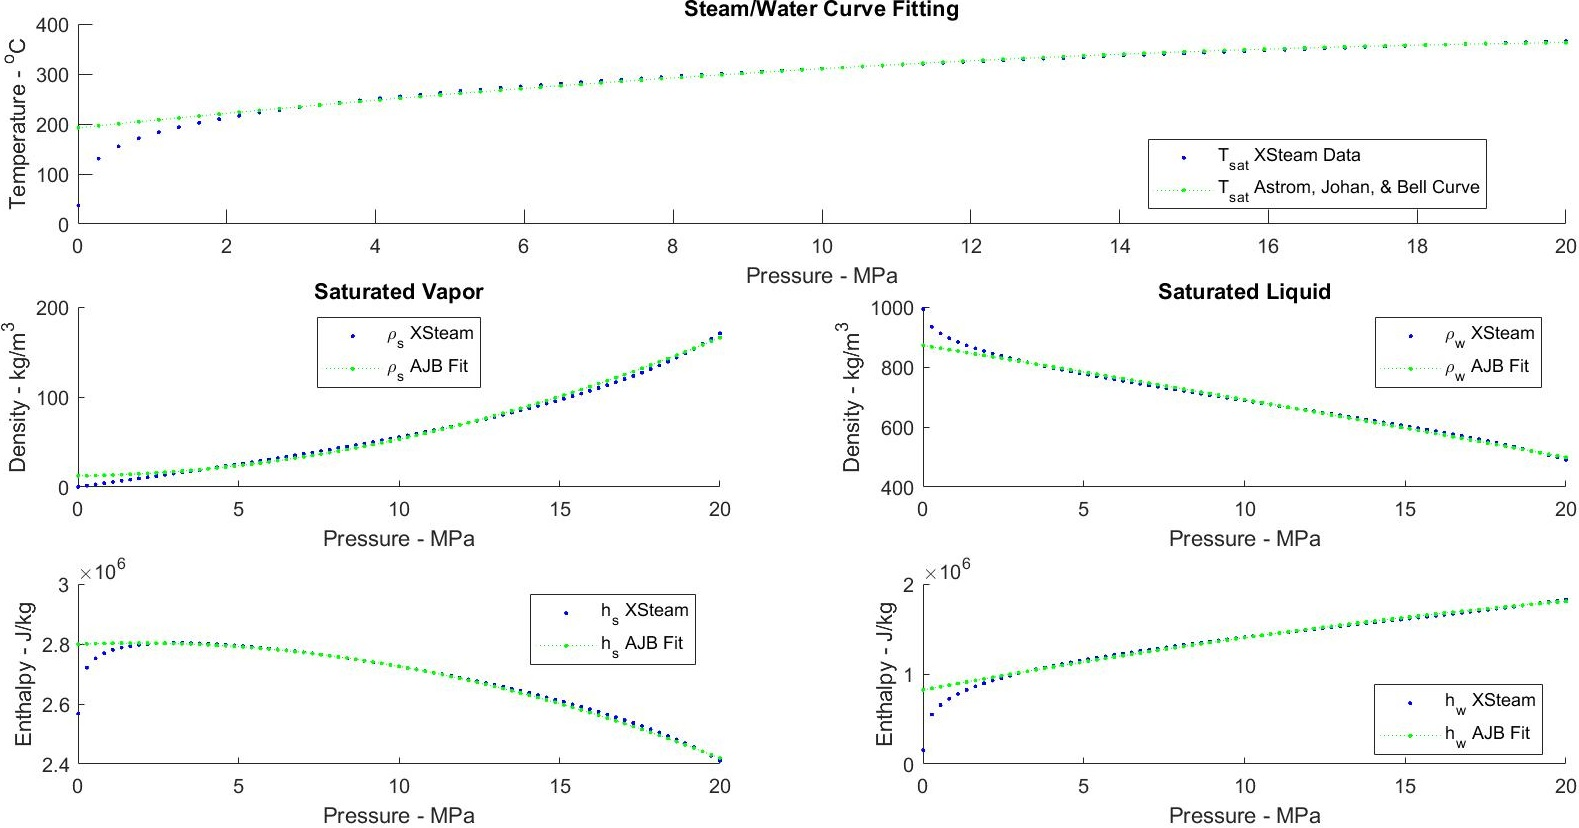
\includegraphics{Modeling/Steam/Steam_Table_Curve_Fits_Original}}
        \caption{Curve Fitting Steam}
        \label{fig:Curve_Fit_SteamA}
        \end{center}
    \end{figure}
    
    A more elaborate model can be used, and a curve fitting process can be applied to the tables of physical properties. The advantage of using a more elaborate model is that the operating parameters can be further expanded outside of the range of where the quadratic model breaks down. The various model types are defined in Table \ref{table:Steam_ModelingB}. Exponential and cubic equations were used for a more accurate fit. Figure \ref{fig:Curve_Fit_SteamB} shows the steam properties table, the quadratic model, and an expanded model. 
    
    \begin{figure}[ht]
        \begin{center}
        \resizebox{\ScaleMLFigSteam \textwidth}{!}{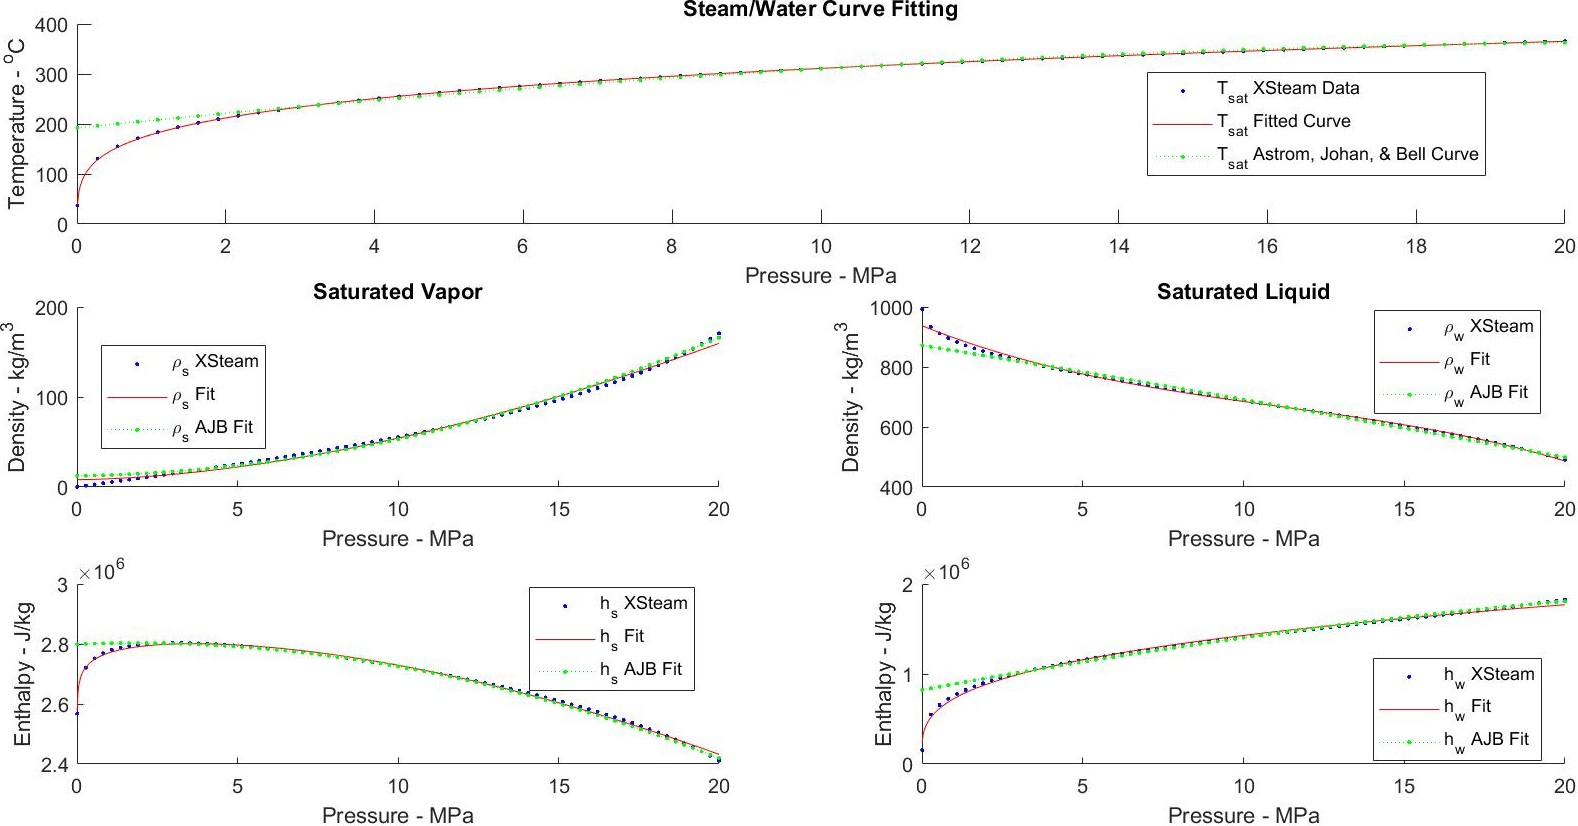
\includegraphics{Modeling/Steam/Steam_Table_Curve_Fits}}
        \caption{Curve Fitting Steam}
        \label{fig:Curve_Fit_SteamB}
        \end{center}
    \end{figure}
    
    \begin{table}[ht]
        \begin{center}
        \begin{scriptsizetabular}{|l| c l l|}
            \hline
              & & Original Model Equation & Expanded Model Equation \\
            \hline
            Saturated Steam Temperature & & $T(p)      = C p^2 + B p + A$ & $T(p)      = Bp^C +A$\\ 
            Saturated Vapor Enthalpy    & & $h_s(p)    = C p^2 + B p + A$ & $h_s(p)    = Dp^E + Bp^C+A$\\ 
            Saturated Vapor Density     & & $\rho_s(p) = C p^2 + B p + A$ & $\rho_s(p) = Bp^C +A$\\ 
            Saturated Liquid Enthalpy   & & $h_w(p)    = C p^2 + B p + A$ & $h_w(p)    = Bp^C +A$\\ 
            Saturated Liquid Density    & & $\rho_w(p) = C p^2 + B p + A$ & $\rho_w(p) = Dp^3 + C p^2 + B p + A$ \\
            \hline
        \end{scriptsizetabular}
        \caption{Expanded Steam Table Models}
        \label{table:Steam_ModelingB}
        \end{center}
    \end{table}    
    
    It is clear from Figure \ref{fig:Curve_Fit_SteamB} that the more complex exponential models are a better fit than the quadratic modeling, as the model does not break down in the lower pressure ranges. While the original quadratic model makes the math much simpler when performing the partial derivatives the use of computational tools (MatLab's Symbolic Toolbox) makes this a rewarding design trade off when compared to the expanded pressure ranges that the new model can operate at and the trivial nature of calculating these partial derivatives. 
    
\section{\r{A}str\"{o}m and Bell Model}

    \r{A}str\"{o}m and Bell's goal in creating a model was to find a moderately complex nonlinear model that captured the key properties of shrink and swell for drum boiler level. A first order model can be used if drum level is considered well controlled. The first order model ignores the drum level and therefore cannot be used for the purposes of this paper. \cite{Astrom}
    
    \subsection{Global Mass and Energy Balance}
    
        The global Mass balance is: 
        $$\frac{\mathrm{d} }{\mathrm{d} t}\left [ \rho_s V_{st} + \rho_w V_{wt}\right ] = q_f - q_s$$\cite{Astrom}
        This can be placed into words as the sum of the change in the mass of the steam and water in the system (calculated as $m = \rho V$) must be equal to the sum of the mass flow rate of the steam flow out of the system and feed-water flow into the system. This is the principle of the conservation of mass. 
        
        The global mass balance can be placed into matrix form with some manipulations to become Eq. \eqref{eq:Mass_Balance} noting that $\rho$ is a function of $p$. \cite{Astrom}
        \begin{equation}
            \label{eq:Mass_Balance}
            \left [ \begin{matrix} e_{11}& e_{12}\end{matrix} \right ] \frac{\mathrm{d} }{\mathrm{d} t} \left [ \begin{matrix} V_{wt}\\ p\end{matrix} \right ] = q_f  - q_s
        \end{equation}
        In Eq. \ref{eq:Mass_Balance} the coefficients are defined as follows:
        \begin{equation*}
                e_{11}      = \rho_w - \rho_s
        \end{equation*}
        \begin{equation*}
                e_{12}      = V_{wt} \frac{\partial \rho_w }{\partial p} - V_{st} \frac{\partial \rho_s }{\partial p}
        \end{equation*}
        
        The global energy balance is 
        $$\frac{\mathrm{d} }{\mathrm{d} t}\left [ \rho_s h_s V_{st} + \rho_w h_w V_{wt} - pV_t + m_tC_pt_m\right ] = Q + q_f h_f - q_s h_s $$\cite{Astrom}
        This can be placed into words as the change of internal energy in both steam and water and the change of energy due to the change in volume and the temperature of the metal must equal the sum of the heat transfer in, the energy the steam brings, and the energy the feed-water brings. 
        
        The global energy balance can be simplified to become:\cite{Astrom}
        \begin{equation}
            \label{eq:Energy_Balance}
            \left [ \begin{matrix} e_{21}& e_{22}\end{matrix} \right ] \frac{\mathrm{d} }{\mathrm{d} t} \left [ \begin{matrix} V_{wt}\\ p\end{matrix} \right ] = Q + q_f h_f  - q_s h_s 
        \end{equation}
        In Eq \ref{eq:Energy_Balance} the coefficients are defined as follows:
        \begin{equation*}
            e_{21} = \rho_w h_w - \rho_s h_s 
        \end{equation*}
        \begin{equation*}
            e_{22} = V_{wt} \left ( h_w  \frac{\partial \rho_w }{\partial p} + \rho_w \frac{\partial h_w }{\partial p}\right ) + V_{st} \left ( h_s  \frac{\partial \rho_s }{\partial p} + \rho_s \frac{\partial h_s }{\partial p}\right ) - V_{t} + m_t C_p \frac{\partial t_s }{\partial p}
        \end{equation*}
        
        %It should be noted that for Mass and Energy balance alone, Equations \eqref{eq:Mass_Balance}-\eqref{eq:Energy_Balance} are enough to create a simple model, however this model is not sufficient to capture the drum level dynamics. 
        %\begin{equation}
        %    \label{eq:Mass_Energy_BalanceA}
        %    \left [ \begin{matrix} e_{11}& e_{12} \\ e_{21}& e_{22}\end{matrix} \right ] \frac{\mathrm{d} }{\mathrm{d} t} \left [ \begin{matrix} V_{wt}\\ p\end{matrix} \right ] =  \left [ \begin{matrix} q_f  - q_s \\ Q + q_f h_f  - q_s h_s \end{matrix} \right ]
        %\end{equation}        
        
        %For future calculations, the Mass and Energy Balance equations \eqref{eq:Mass_Energy_BalanceA} will be expanded trivially into Equation \eqref{eq:Mass_Energy_Balance}. Please note that $\alpha_r$ and $V_{sd}$ will be defined as states and used later. 
        %\begin{equation}
        %    \label{eq:Mass_Energy_Balance}
        %    \left [ \begin{matrix} e_{11}& e_{12} & 0& 0\\ e_{21}& e_{22}& 0& 0\end{matrix} \right ] %\frac{\mathrm{d} }{\mathrm{d} t} \left [ \begin{matrix} V_{wt}\\ p\\ \alpha_r\\ V_{sd}\end{matrix} %\right ] =  \left [ \begin{matrix} q_f  - q_s \\ Q + q_f h_f  - q_s h_s \end{matrix} \right ]
        %\end{equation}           

    \subsection{Distribution of Steam in Risers and Drum}
    
    
        The energy balance for the riser section:
        $$\frac{\mathrm{d} }{\mathrm{d} t}\left [ \rho_s h_s \overline{\alpha}_v V_{r} + \rho_w h_w\left ( 1 - \overline{\alpha}_v \right ) V_{r} - pV_r + m_r C_p t_s\right ] = Q + q_{dc} h_w - \left ( \alpha_r h_c + h_w \right )q_{r} $$\cite{Astrom}
        This can be placed into words as the change of internal energy in both steam and water in the risers and the change of energy due to the change in volume and the temperature of the metal of the risers  must equal the sum of the heat transfer in, the energy the risers looses, and the energy the water in the down comers brings. $\overline{\alpha}_v$ is the average steam volume ratio.
        
        The riser section energy balance can be simplified to become:\cite{Astrom}
        \begin{equation}
            \label{eq:Riser_Energy_Balance}
            \left [ \begin{matrix}  e_{32}& e_{33}\end{matrix} \right ] \frac{\mathrm{d} }{\mathrm{d} t} \left [ \begin{matrix}  p\\ \alpha_r\end{matrix} \right ] = Q + \alpha_r h_c q_{dc} 
        \end{equation}
        
        \clearpage
    
        In Eq \ref{eq:Riser_Energy_Balance} the coefficients are defined as follows:
        
        
        
        \begin{equation*}
            \aligned
                e_{32}  =& \left ( \rho_w \frac{\partial h_w }{\partial p} + \rho_s \frac{\partial h_s }{\partial p}\right )\left ( 1-\overline{\alpha}_v \right )V_r + \left ( \left ( 1- \alpha_r \right ) h_c \frac{\partial \rho_s }{\partial p} + \rho_s \frac{\partial h_s }{\partial p} \right ) \overline{\alpha}_v V_r \\
                         &+  \left (  \rho_s + \left ( \rho_w - \rho_s \right )\alpha_r \right ) h_c V_r \frac{\partial \overline{\alpha}_v }{\partial p}  - V_r+m_r C_p \frac{\partial t_s }{\partial p}
                \endaligned
        \end{equation*}
        

        \begin{equation*}
            e_{33}  = \left ( \left ( 1-\alpha_r \right )\rho_s + \alpha_r \rho_w \right )h_c V_r \frac{\partial \overline{\alpha}_v }{\partial \alpha_r} 
        \end{equation*}
        
        The mass balance for the riser section is:
        $$\frac{\mathrm{d} }{\mathrm{d} t}\left [ \rho_s \overline{\alpha}_v V_{r} + \rho_w \left ( 1 - \overline{\alpha}_v \right )V_{r} \right ] = q_{dc}-q_{r} $$\cite{Astrom}
        This can be placed into words as the change in density and volume of both steam and water in the risers must be equal to the mass flow rate of the sum of the mass flow rates into the down comers and out of the risers.  
        
        The riser section mass balance can be simplified to become:
        \begin{equation}
            \label{eq:Riser_Mass_Balance}
            \left [ \begin{matrix}  e_{42}& e_{43}& e_{44}\end{matrix} \right ] \frac{\mathrm{d} }{\mathrm{d} t} \left [ \begin{matrix} p\\ \alpha_r\\ V_{sd}\end{matrix} \right ] = \frac{\rho_s}{T_d}  \left ( V_{sd}^0  - V_{sd}\right ) + \frac{h_f - h_w}{h_c}q_f
        \end{equation}
        
        In Eq \ref{eq:Riser_Mass_Balance} the coefficients are defined as follows:\cite{Astrom}

        
        \begin{equation*}
            \aligned
                e_{42} = & V_{sd}\frac{\partial \rho_s }{\partial p} + \frac{1}{h_c}\left ( \rho_s V_{sd} \frac{\partial h_s }{\partial p} + \rho_w V_{wd} \frac{\partial h_w }{\partial p} - V_{sd} - V_{wd} + m_d C_p \frac{\partial t_s }{\partial p} \right ) \\
                &+ \alpha_r\left ( 1+\beta \right )V_r \left ( \overline{\alpha}_v \frac{\partial \rho_s }{\partial p} + \left ( 1-\overline{\alpha}_v \right )\frac{\partial \rho_w }{\partial p} + \left ( \rho_s - \rho_w \right ) \frac{\partial \overline{\alpha}_v }{\partial p} \right )
            \endaligned
        \end{equation*}
        

        \begin{equation*}
            e_{43} = \alpha_r\left ( 1+\beta \right )\left ( \rho_s - \rho_w \right )V_r\frac{\partial \overline{\alpha}_v }{\partial p}
        \end{equation*}
        \begin{equation*}    
            e_{44} = \rho_s
        \end{equation*}

\section{Simulation of \r{A}str\"{o}m and Bell Model}
    
    Equations \ref{eq:Mass_Balance}, \ref{eq:Energy_Balance}, \ref{eq:Riser_Energy_Balance}, and  \ref{eq:Riser_Mass_Balance} can be combined to give the following equation :

    $$\left [ \begin{matrix}e_{11}& e_{12}& 0& 0 \\ e_{21}& e_{22}& 0& 0 \\ 0 & e_{32}& e_{33}& 0 \\ 0 & e_{42}& e_{43}& e_{44}\end{matrix} \right ] \frac{\mathrm{d} }{\mathrm{d} t} \left [ \begin{matrix} V_{wt}\\ p\\ \alpha_r\\ V_{sd}\end{matrix} \right ] = \left [ \begin{matrix} q_f  - q_s \\ Q + q_f h_f  - q_s h_s\\ Q + \alpha_r h_c q_{dc} \\ \frac{\rho_s}{T_d}  \left ( V_{sd}^0  - V_{sd}\right ) + \frac{h_f - h_w}{h_c}q_f \end{matrix} \right ]$$

    \begin{equation}
        \label{eq:Model_1}
        \frac{\mathrm{d} }{\mathrm{d} t} \left [ \begin{matrix} V_{wt}\\ p\\ \alpha_r\\ V_{sd}\end{matrix} \right ] =
        \left [ \begin{matrix}e_{11}& e_{12}& 0& 0 \\ e_{21}& e_{22}& 0& 0 \\ 0 & e_{32}& e_{33}& 0 \\ 0 & e_{42}& e_{43}& e_{44}\end{matrix} \right ] ^{-1} \left [ \begin{matrix} q_f  - q_s \\ Q + q_f h_f  - q_s h_s\\ Q + \alpha_r h_c q_{dc} \\ \frac{\rho_s}{T_d}  \left ( V_{sd}^0  - V_{sd}\right ) + \frac{h_f - h_w}{h_c}q_f \end{matrix} \right ]
    \end{equation}
    
    This can be considered a nonlinear state space model, which takes the form of 
    $$\dot{x}(t) = F\left ( x(t),u(t) \right )$$
    Where Eq \ref{eq:Model_1} uses the following as states:
    $$ \begin{matrix} V_{wt} & p& \alpha_r& V_{sd}\end{matrix} $$
    and where Eq \ref{eq:Model_1} uses the following as Inputs:
    $$ \begin{matrix} q_f & q_s & Q & t_f\end{matrix} $$
    
    For purposes of boiler control, the two requested outputs to be predicted are drum level and drum pressure, both of which may be measured directly using simple sensors. The Nonlinear State Space output equation takes the following form: 
    $$y(t) = G\left ( x(t),u(t) \right )$$
    where the control outputs can be calculated as seen in Equation \ref{eq:Model_1_output}. Where $V_{wd}$ is a known function of the states and inputs and $A_d$ is a constant. 
    \begin{equation}
        \label{eq:Model_1_output}
        y(t) = \left [ \begin{matrix} l\\ p \end{matrix} \right ] = \left [ \begin{matrix} \frac{V_{sd} + V_{wd}}{A_d}\\ p \end{matrix} \right ]= \left [ \begin{matrix} \frac{x_4 + V_{wd}}{A_d}\\ x_2 \end{matrix} \right ]
    \end{equation}
    
    If access to all of the states is possible, it allows for calculations of far more outputs. These include: the level contributions from both steam and water, riser and down comer mass flow rate, total water volume, volume of steam in the drum, condensation flow rate, and the average steam volume ratio. These values are of interest, as they give insight into the boiler dynamics, however they are not required for control. The expanded output equations can be seen below:
    $$y_{expanded}(t) = \left [ \begin{matrix} l\\ p \\ \vdots \end{matrix} \right ] $$
    
    \subsection{Equilibrium Values}
    
        To find the equilibrium point of the system, Eq \ref{eq:Model_1} is set to 0. Then from an operating point, the equations are solved.
        
        The operating point chosen are:
        $$ \begin{matrix} V_{wt0}     & = &   57.1 & & & Q_{0}  & = & 86.78\\ 
                          p_0         & = &    8.5 & & & q_{f0} & = & 50.8\\ 
                          \alpha_{r0} & = & 0.0524 & & & t_{f0} & = & 247.66\\ 
                          V_{sd0}     & = &    4.9 & & & q_{s0} & = & 50.8
                          \end{matrix} $$
                  
    \subsection{Comparison of simulation and \r{A}str\"{o}m and Bell's previous work}

        Validation of the reproduced \r{A}str\"{o}m and Bell model was done by simulating step inputs of the model used in Eq. \eqref{eq:Model_1} and comparing the results to the results of the simulated step inputs that \r{A}str\"{o}m and Bell published. 
        
        The following figures were taken from \r{A}str\"{o}m and Bell's paper, section 5. These are used to directly compare the model generated matches the model, as not all parameters were given. 
        
        % Figure 4 Caption: Responses to a step corresponding to 10 MW in fuel flow rate at medium load
        % Figure 5 Caption: Responses to a step change of 10 kg/s in steam flow rate at medium load
        % Figure 6 Caption: Responses to a step corresponding to 10 MW in fuel flow rate at medium (solid) and high (dashed) loads
        % Figure 7 Caption: Responses to a step change of 10 kg/s in steam flow rate at medium (solid) and high (dashed) loads
        % Figure 8 Caption: Responses to a step change of 10 kg/s in feed water flow rate at medium (solid) and high (dashed) loads
        % Figure 9 Caption: Responses to a step change of 10$^O$ C in feed water temperature at medium (solid) and high (dashed) loads
        
        10 MW fuel flow Step Responses: Figures \ref{fig:Fig6A} - \ref{fig:Fig4D}
        
        \begin{figure}[ht]
            \begin{center}
                \resizebox{\ScaleABFigThree \textwidth}{!}{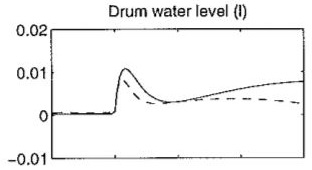
\includegraphics{Modeling/4State/AB_Figures/Figure6/Figure6-AB-1}}
                
                Figure 6 from \r{A}str\"{o}m and Bell's paper, section 5 \cite{Astrom}
                
                \resizebox{\ScaleMLFigThree \textwidth}{!}{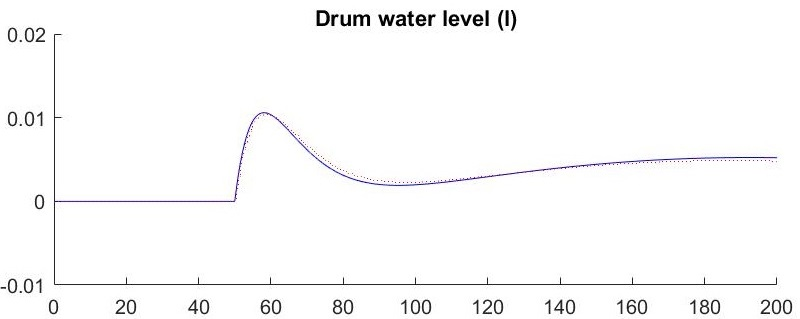
\includegraphics{Modeling/4State/Matlab/Figure12/Figure12-1}}
                
                Simulation Results using Model from Eq \eqref{eq:Model_1}
                
                \caption{Drum Water Level Response to a step corresponding to 10 MW in fuel flow rate}
                \label{fig:Fig6A}
                
            \end{center}
        \end{figure}  % Level
        \begin{figure}[ht]
            \begin{center}
                 \resizebox{\ScaleABFigThree \textwidth}{!}{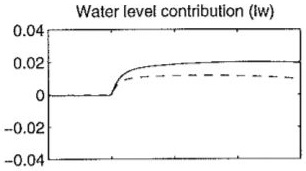
\includegraphics{Modeling/4State/AB_Figures/Figure6/Figure6-AB-3}}
                
                Figure 6 from \r{A}str\"{o}m and Bell's paper, section 5 \cite{Astrom}

                \resizebox{\ScaleMLFigThree \textwidth}{!}{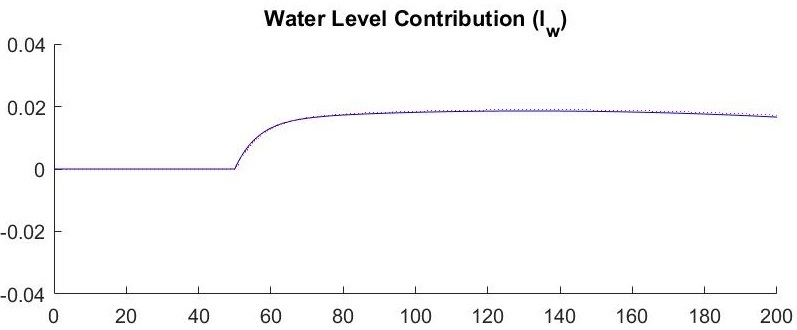
\includegraphics{Modeling/4State/Matlab/Figure12/Figure12-3}}
                
                Simulation Results using Model from Eq \eqref{eq:Model_1}
                
                \caption{Water Level Contribution to a step corresponding to 10 MW in fuel flow rate}
                \label{fig:Fig6B}
            \end{center}
        \end{figure}  % Level Water Contribution
        \begin{figure}[ht]
            \begin{center}
                \resizebox{\ScaleABFigThree \textwidth}{!}{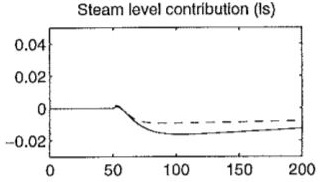
\includegraphics{Modeling/4State/AB_Figures/Figure6/Figure6-AB-5}}
                
                Figure 6 from \r{A}str\"{o}m and Bell's paper, section 5 \cite{Astrom}    
                
                \resizebox{\ScaleMLFigThree \textwidth}{!}{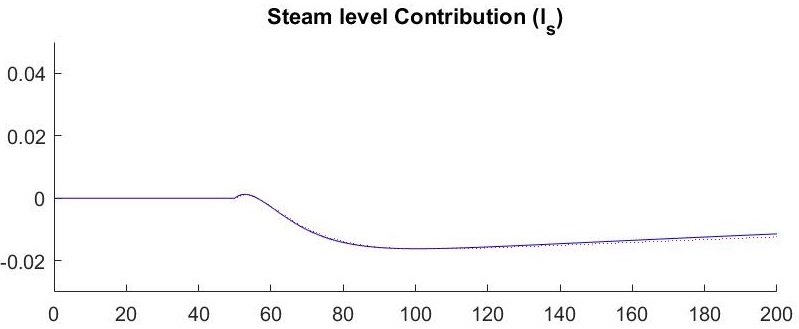
\includegraphics{Modeling/4State/Matlab/Figure12/Figure12-5}}
                
                Simulation Results using Model from Eq \eqref{eq:Model_1}
                
                \caption{Steam Level Contribution to a step corresponding to 10 MW in fuel flow rate}
                \label{fig:Fig6C}
            \end{center}
        \end{figure}  % Level Steam Contribution    
            
        \begin{figure}[ht]
            \begin{center}
                \resizebox{\ScaleABFigThree \textwidth}{!}{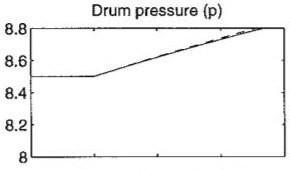
\includegraphics{Modeling/4State/AB_Figures/Figure6/Figure6-AB-2}}
                
                Figure 6 from \r{A}str\"{o}m and Bell's paper, section 5 \cite{Astrom}
                    
                \resizebox{\ScaleMLFigThree \textwidth}{!}{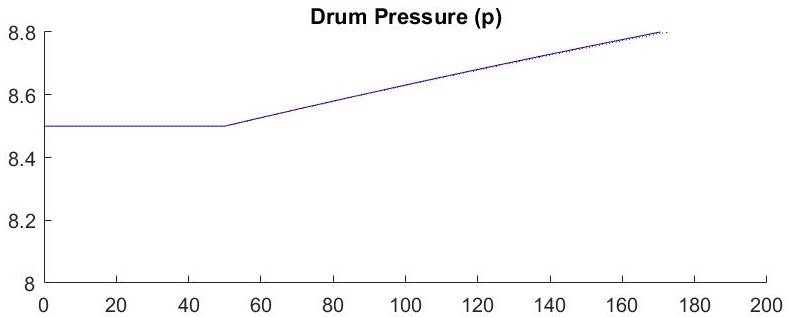
\includegraphics{Modeling/4State/Matlab/Figure12/Figure12-2}}
                
                Simulation Results using Model from Eq \eqref{eq:Model_1}
                
                \caption{Drum Pressure Response to a step corresponding to 10 MW in fuel flow rate}
                \label{fig:Fig6D}                
            \end{center}
        \end{figure}  % Drum Pressure
        \begin{figure}[ht]
            \begin{center}
                \resizebox{\ScaleABFigThree \textwidth}{!}{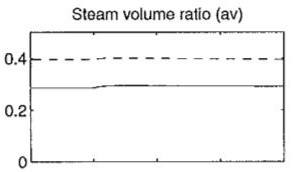
\includegraphics{Modeling/4State/AB_Figures/Figure6/Figure6-AB-4}}
                    
                Figure 6 from \r{A}str\"{o}m and Bell's paper, section 5 \cite{Astrom}
                
                \resizebox{\ScaleMLFigThree \textwidth}{!}{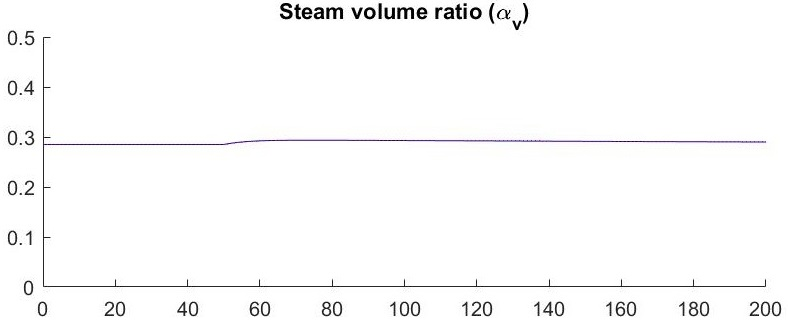
\includegraphics{Modeling/4State/Matlab/Figure12/Figure12-4}}
                
                Simulation Results using Model from Eq \eqref{eq:Model_1}
                
                \caption{Steam Volume Ratio Response to a step corresponding to 10 MW in fuel flow rate}
                \label{fig:Fig6E}
            \end{center}
        \end{figure}  % Steam Volume Ratio 
        \begin{figure}[ht]
            \begin{center}
                \resizebox{\ScaleABFigThree \textwidth}{!}{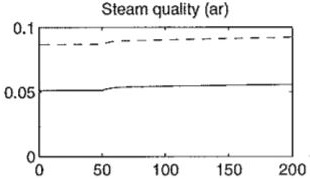
\includegraphics{Modeling/4State/AB_Figures/Figure6/Figure6-AB-6}}
                
                Figure 6 from \r{A}str\"{o}m and Bell's paper, section 5 \cite{Astrom}    
                
                \resizebox{\ScaleMLFigThree \textwidth}{!}{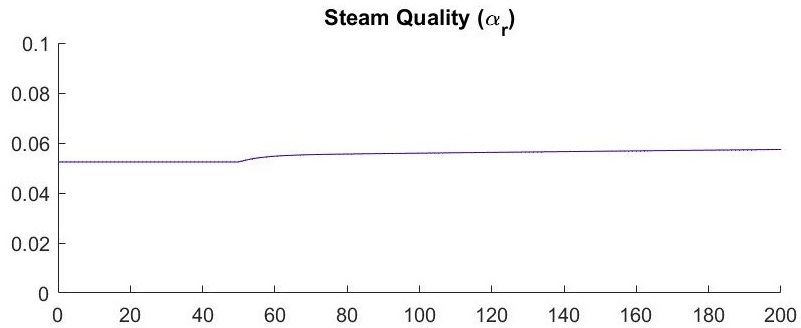
\includegraphics{Modeling/4State/Matlab/Figure12/Figure12-6}}
                
                Simulation Results using Model from Eq \eqref{eq:Model_1}
                
                \caption{Steam Quality Response to a step corresponding to 10 MW in fuel flow rate}
                \label{fig:Fig6F}
            \end{center}
        \end{figure}  % Steam Quality

        \begin{figure}[ht]
            \begin{center}
                \resizebox{\ScaleABFigThree \textwidth}{!}{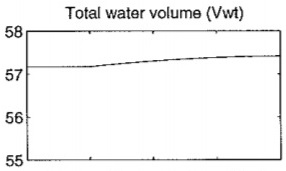
\includegraphics{Modeling/4State/AB_Figures/Figure4/Figure4-AB-2}}
                
                Figure 4 from \r{A}str\"{o}m and Bell's paper, section 5 \cite{Astrom}    
                
                \resizebox{\ScaleMLFigThree \textwidth}{!}{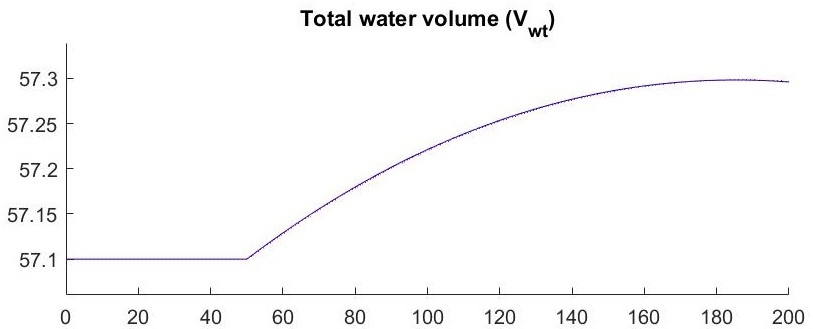
\includegraphics{Modeling/4State/Matlab/Figure11/Figure11-2}}
                
                Simulation Results using Model from Eq \eqref{eq:Model_1}
                
                \caption{Total Water Volume Response to a step corresponding to 10 MW in fuel flow rate}
                \label{fig:Fig4A}
            \end{center}
        \end{figure}
        \begin{figure}[ht]
            \begin{center}
                \resizebox{\ScaleABFigThree \textwidth}{!}{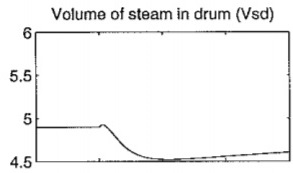
\includegraphics{Modeling/4State/AB_Figures/Figure4/Figure4-AB-4}}
                
                Figure 4 from \r{A}str\"{o}m and Bell's paper, section 5 \cite{Astrom}    
                
                \resizebox{\ScaleMLFigThree \textwidth}{!}{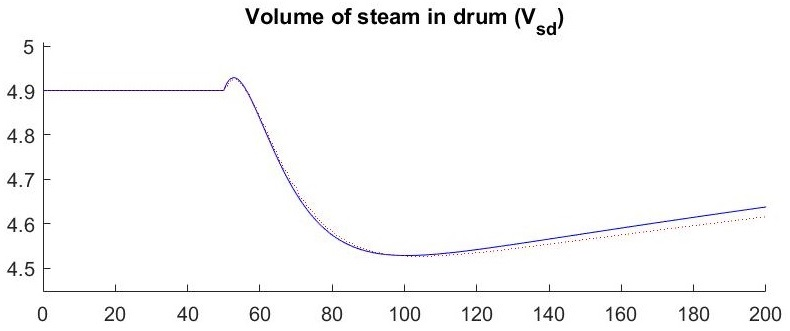
\includegraphics{Modeling/4State/Matlab/Figure11/Figure11-4}}
                
                Simulation Results using Model from Eq \eqref{eq:Model_1}
                
                \caption{Volume of Steam in Drum Response to a step corresponding to 10 MW in fuel flow rate}
                \label{fig:Fig4B}                
            \end{center}
        \end{figure}
        \begin{figure}[ht]
            \begin{center}
                \resizebox{\ScaleABFigThree \textwidth}{!}{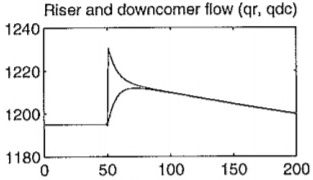
\includegraphics{Modeling/4State/AB_Figures/Figure4/Figure4-AB-5}}
                
                Figure 4 from \r{A}str\"{o}m and Bell's paper, section 5 \cite{Astrom}    
                
                \resizebox{\ScaleMLFigThree \textwidth}{!}{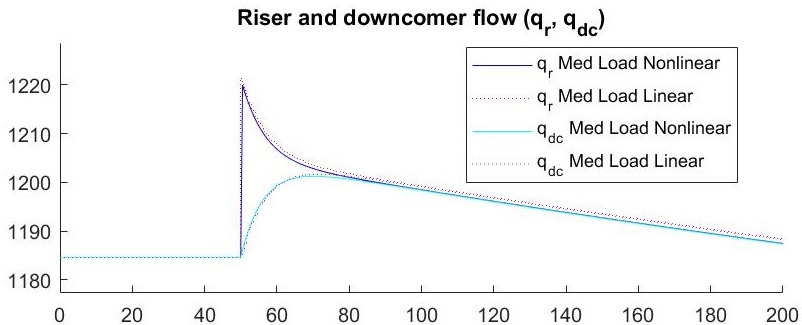
\includegraphics{Modeling/4State/Matlab/Figure11/Figure11-5}}
                
                Simulation Results using Model from Eq \eqref{eq:Model_1}
                
                \caption{Riser and Downcomer Flow Response to a step corresponding to 10 MW in fuel flow rate}
                \label{fig:Fig4C}
            \end{center}
        \end{figure}
        \begin{figure}[ht]
            \begin{center}
                \resizebox{\ScaleABFigThree \textwidth}{!}{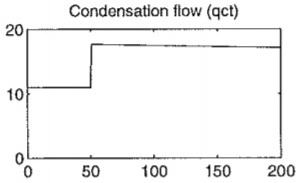
\includegraphics{Modeling/4State/AB_Figures/Figure4/Figure4-AB-6}}
                
                Figure 4 from \r{A}str\"{o}m and Bell's paper, section 5 \cite{Astrom}
                
                \resizebox{\ScaleMLFigThree \textwidth}{!}{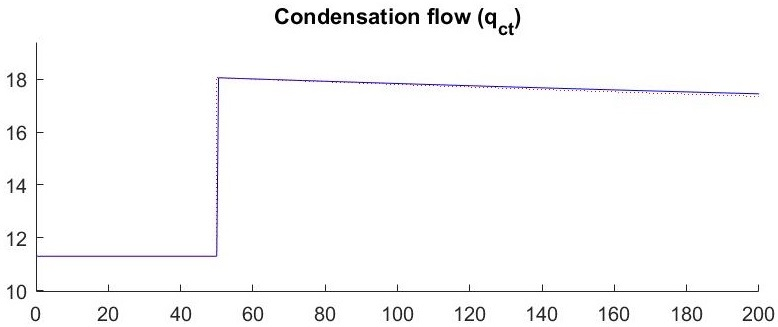
\includegraphics{Modeling/4State/Matlab/Figure11/Figure11-6}}
                
                Simulation Results using Model from Eq \eqref{eq:Model_1}
                
                \caption{Condensation Flow Response to a step corresponding to 10 MW in fuel flow rate}
                \label{fig:Fig4D}
            \end{center}
        \end{figure}            
        
        10 kg/s in steam flow Step Responses: Figures \ref{fig:Fig7A} - \ref{fig:Fig5D}
        \begin{figure}[ht]
            \begin{center}
                \resizebox{\ScaleABFigThree \textwidth}{!}{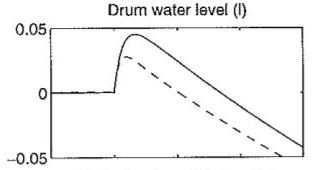
\includegraphics{Modeling/4State/AB_Figures/Figure7/Figure7-AB-1}}
                
                Figure 7 from \r{A}str\"{o}m and Bell's paper, section 5 \cite{Astrom}
                
                \resizebox{\ScaleMLFigThree \textwidth}{!}{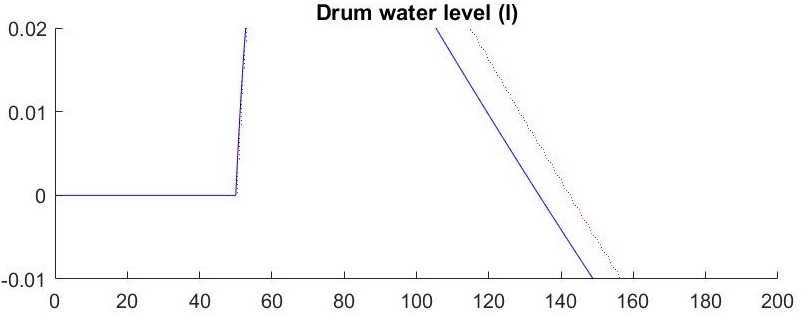
\includegraphics{Modeling/4State/Matlab/Figure22/Figure22-1}}
                
                Simulation Results using Model from Eq \eqref{eq:Model_1}
                
                \caption{Drum Water Level Response to a step change of 10 kg/s in steam flow rate}
                \label{fig:Fig7A}
            \end{center}
        \end{figure}  % Level
        \begin{figure}[ht]
            \begin{center}
                \resizebox{\ScaleABFigThree \textwidth}{!}{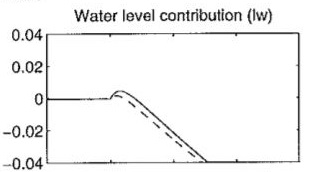
\includegraphics{Modeling/4State/AB_Figures/Figure7/Figure7-AB-3}}
                
                Figure 7 from \r{A}str\"{o}m and Bell's paper, section 5 \cite{Astrom}

                \resizebox{\ScaleMLFigThree \textwidth}{!}{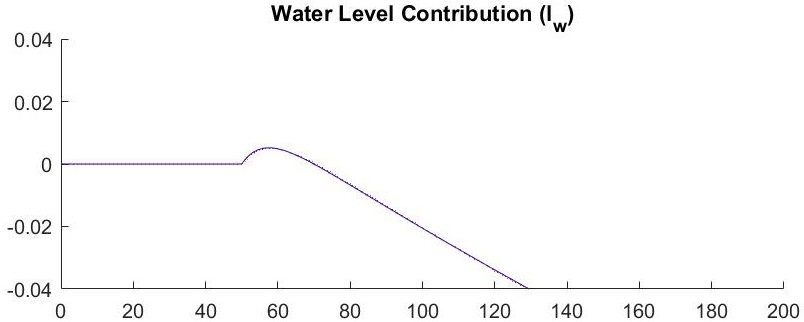
\includegraphics{Modeling/4State/Matlab/Figure22/Figure22-3}}

                Simulation Results using Model from Eq \eqref{eq:Model_1}
                
                \caption{Water Level Contribution to a step change of 10 kg/s in steam flow rate}
                \label{fig:Fig7B}
            \end{center}
        \end{figure}  % Level Water Contribution
        \begin{figure}[ht]
            \begin{center}
                \resizebox{\ScaleABFigThree \textwidth}{!}{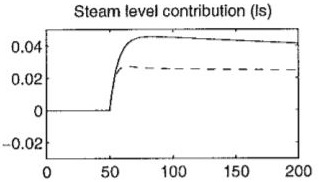
\includegraphics{Modeling/4State/AB_Figures/Figure7/Figure7-AB-5}}
                
                Figure 7 from \r{A}str\"{o}m and Bell's paper, section 5 \cite{Astrom}
                
                \resizebox{\ScaleMLFigThree \textwidth}{!}{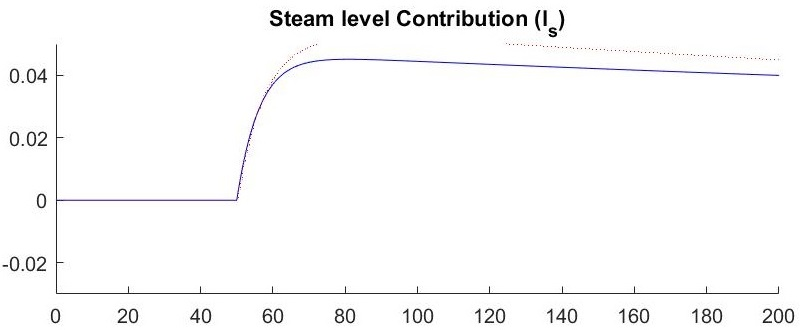
\includegraphics{Modeling/4State/Matlab/Figure22/Figure22-5}}
                
                Simulation Results using Model from Eq \eqref{eq:Model_1}
                
                \caption{Steam Level Contribution to a step change of 10 kg/s in steam flow rate}
                \label{fig:Fig7C}
            \end{center}
        \end{figure}  % Level Steam Contribution    
        
        \begin{figure}[ht]
            \begin{center}
                \resizebox{\ScaleABFigThree \textwidth}{!}{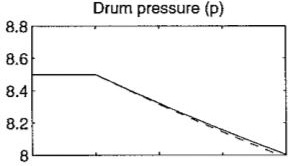
\includegraphics{Modeling/4State/AB_Figures/Figure7/Figure7-AB-2}}
                
                Figure 7 from \r{A}str\"{o}m and Bell's paper, section 5 \cite{Astrom}
                
                \resizebox{\ScaleMLFigThree \textwidth}{!}{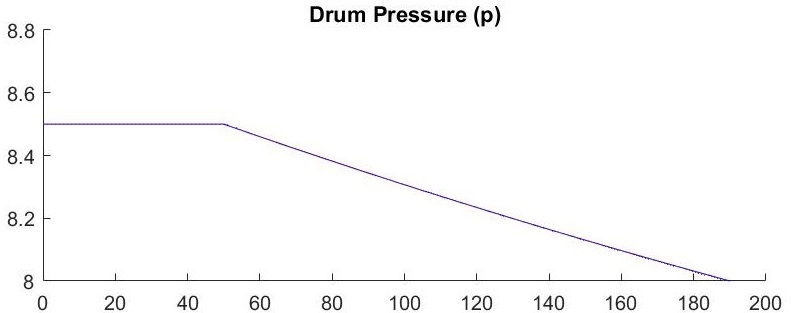
\includegraphics{Modeling/4State/Matlab/Figure22/Figure22-2}}
                
                Simulation Results using Model from Eq \eqref{eq:Model_1}
                
                \caption{Drum Pressure Response to a step change of 10 kg/s in steam flow rate}
                \label{fig:Fig7D}
            \end{center}
        \end{figure}  % Drum Pressure
        \begin{figure}[ht]
            \begin{center}
                \resizebox{\ScaleABFigThree \textwidth}{!}{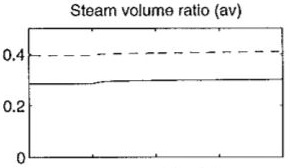
\includegraphics{Modeling/4State/AB_Figures/Figure7/Figure7-AB-4}}
                
                Figure 7 from \r{A}str\"{o}m and Bell's paper, section 5 \cite{Astrom}
                
                \resizebox{\ScaleMLFigThree \textwidth}{!}{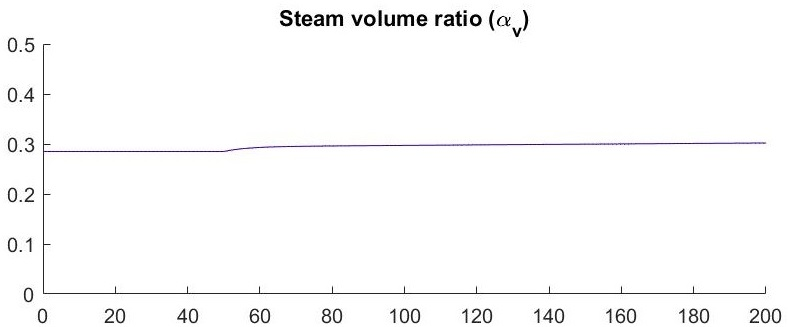
\includegraphics{Modeling/4State/Matlab/Figure22/Figure22-4}}
                
                Simulation Results using Model from Eq \eqref{eq:Model_1}
                
                \caption{Steam Volume Ratio Response to a step change of 10 kg/s in steam flow rate}
                \label{fig:Fig7E}
            \end{center}
        \end{figure}  % Steam Volume Ratio 
        \begin{figure}[ht]
            \begin{center}
                \resizebox{\ScaleABFigThree \textwidth}{!}{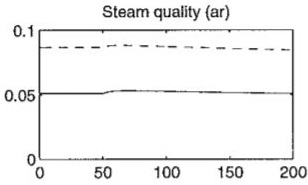
\includegraphics{Modeling/4State/AB_Figures/Figure7/Figure7-AB-6}}
                
                Figure 7 from \r{A}str\"{o}m and Bell's paper, section 5 \cite{Astrom}
                
                \resizebox{\ScaleMLFigThree \textwidth}{!}{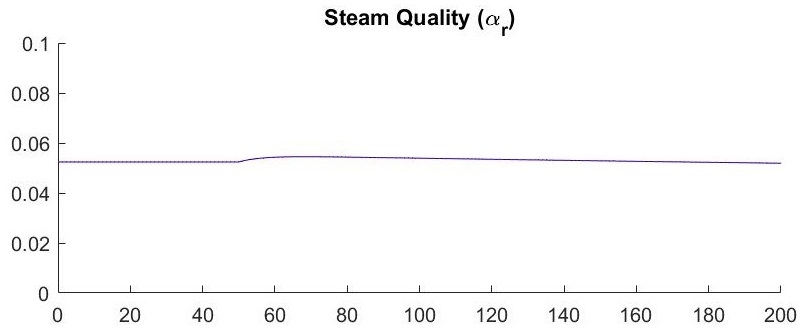
\includegraphics{Modeling/4State/Matlab/Figure22/Figure22-6}}
                
                Simulation Results using Model from Eq \eqref{eq:Model_1}
                
                \caption{Steam Quality Response to a step change of 10 kg/s in steam flow rate}
                \label{fig:Fig7F}
            \end{center}
        \end{figure}  % Steam Quality

        \begin{figure}[ht]
            \begin{center}
                \resizebox{\ScaleABFigThree \textwidth}{!}{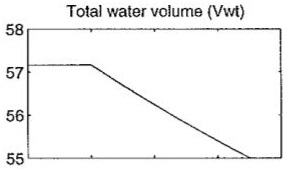
\includegraphics{Modeling/4State/AB_Figures/Figure5/Figure5-AB-2}}
                
                Figure 5 from \r{A}str\"{o}m and Bell's paper, section 5 \cite{Astrom}
                
                \resizebox{\ScaleMLFigThree \textwidth}{!}{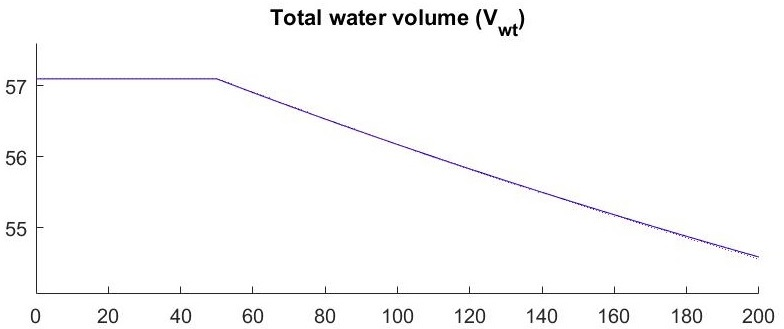
\includegraphics{Modeling/4State/Matlab/Figure21/Figure21-2}}
                
                Simulation Results using Model from Eq \eqref{eq:Model_1}
                
                \caption{Total Water Volume Response to a step change of 10 kg/s in steam flow rate}
                \label{fig:Fig5A}
            \end{center}
        \end{figure}
        \begin{figure}[ht]
            \begin{center}
                \resizebox{\ScaleABFigThree \textwidth}{!}{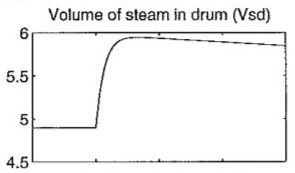
\includegraphics{Modeling/4State/AB_Figures/Figure5/Figure5-AB-4}}
                
                Figure 5 from \r{A}str\"{o}m and Bell's paper, section 5 \cite{Astrom}
                
                \resizebox{\ScaleMLFigThree \textwidth}{!}{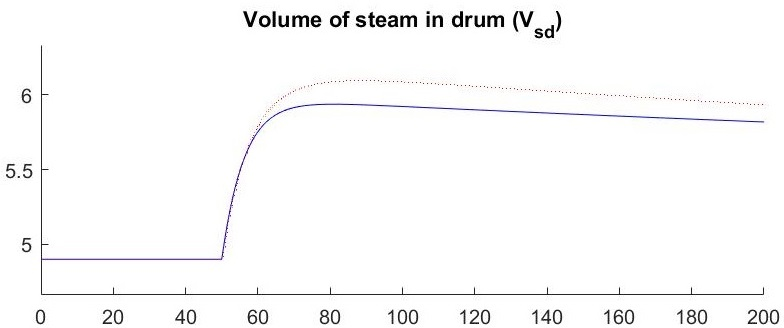
\includegraphics{Modeling/4State/Matlab/Figure21/Figure21-4}}
                
                Simulation Results using Model from Eq \eqref{eq:Model_1}
                
                \caption{Volume of Steam in Drum Response to a step change of 10 kg/s in steam flow rate}
                \label{fig:Fig5B}
            \end{center}
        \end{figure}
        \begin{figure}[ht]
            \begin{center}
                \resizebox{\ScaleABFigThree \textwidth}{!}{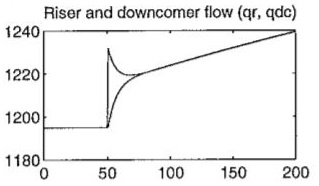
\includegraphics{Modeling/4State/AB_Figures/Figure5/Figure5-AB-5}}
                
                Figure 5 from \r{A}str\"{o}m and Bell's paper, section 5 \cite{Astrom}
                
                \resizebox{\ScaleMLFigThree \textwidth}{!}{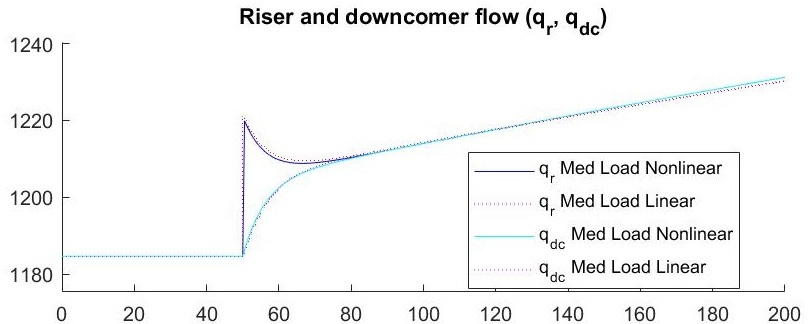
\includegraphics{Modeling/4State/Matlab/Figure21/Figure21-5}}
                
                Simulation Results using Model from Eq \eqref{eq:Model_1}
                
                \caption{Riser and Downcomer Flow Response to a step change of 10 kg/s in steam flow rate}
                \label{fig:Fig5C}
            \end{center}
        \end{figure}
        \begin{figure}[ht]
            \begin{center}
                \resizebox{\ScaleABFigThree \textwidth}{!}{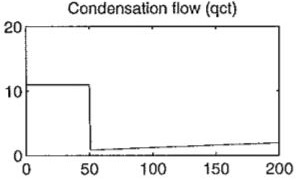
\includegraphics{Modeling/4State/AB_Figures/Figure5/Figure5-AB-6}}
                
                Figure 5 from \r{A}str\"{o}m and Bell's paper, section 5 \cite{Astrom}
                
                \resizebox{\ScaleMLFigThree \textwidth}{!}{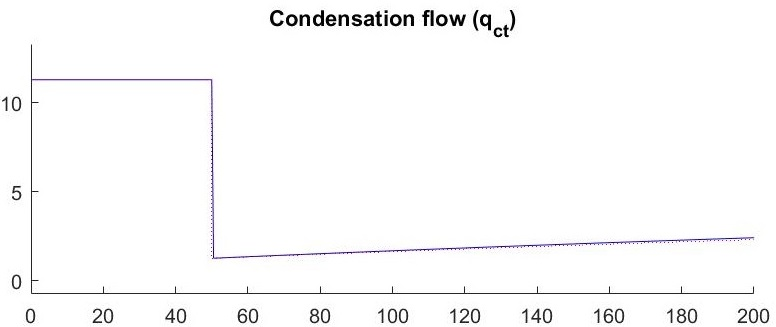
\includegraphics{Modeling/4State/Matlab/Figure21/Figure21-6}}
                
                Simulation Results using Model from Eq \eqref{eq:Model_1}
                
                \caption{Condensation Flow Response to a step change of 10 kg/s in steam flow rate}
                \label{fig:Fig5D}
            \end{center}
        \end{figure}     
            
        10 kg/s in feed water flow Step Responses: Figures \ref{fig:Fig8A}-\ref{fig:Fig8F}
        \begin{figure}[ht]
            \begin{center}
                \resizebox{\ScaleABFigThree \textwidth}{!}{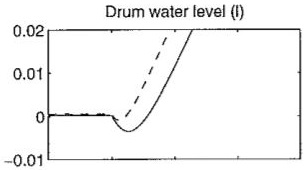
\includegraphics{Modeling/4State/AB_Figures/Figure8/Figure8-AB-1}}
                
                Figure 8 from \r{A}str\"{o}m and Bell's paper, section 5 \cite{Astrom}
                
                \resizebox{\ScaleMLFigThree \textwidth}{!}{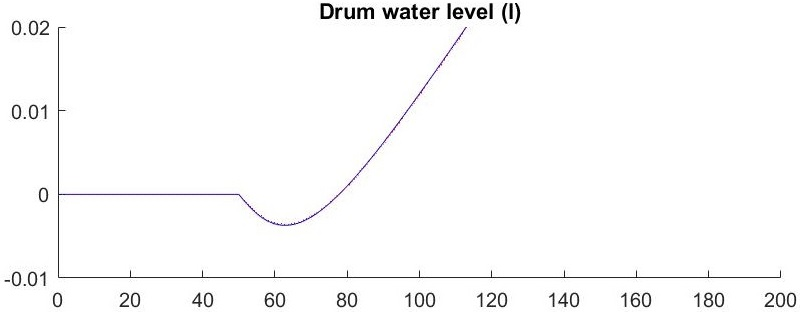
\includegraphics{Modeling/4State/Matlab/Figure32/Figure32-1}}
                
                Simulation Results using Model from Eq \eqref{eq:Model_1}
                
                \caption{Drum Water Level Response to a step corresponding to 10 kg/s in feed water flow rate}
                \label{fig:Fig8A}
            \end{center}
        \end{figure}  % Level
        \begin{figure}[ht]
            \begin{center}
                \resizebox{\ScaleABFigThree \textwidth}{!}{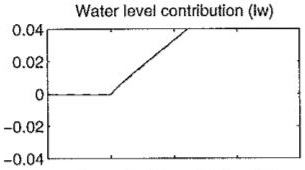
\includegraphics{Modeling/4State/AB_Figures/Figure8/Figure8-AB-3}}
                
                Figure 8 from \r{A}str\"{o}m and Bell's paper, section 5 \cite{Astrom}
                
                \resizebox{\ScaleMLFigThree \textwidth}{!}{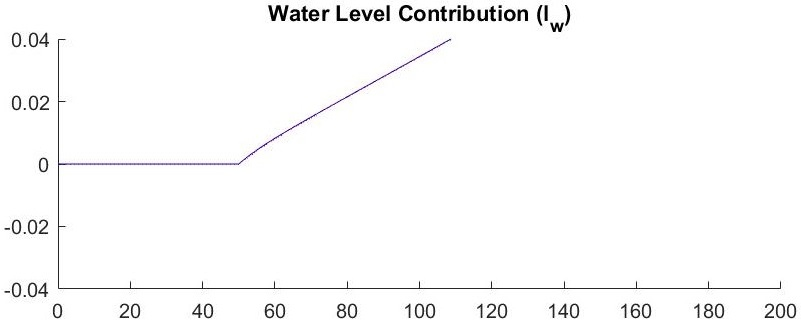
\includegraphics{Modeling/4State/Matlab/Figure32/Figure32-3}}
                
                Simulation Results using Model from Eq \eqref{eq:Model_1}
                
                \caption{Water Level Contribution to a step corresponding to 10 kg/s in feed water flow rate}
                \label{fig:Fig8B}
            \end{center}
        \end{figure}  % Level Water Contribution
        \begin{figure}[ht]
            \begin{center}
                \resizebox{\ScaleABFigThree \textwidth}{!}{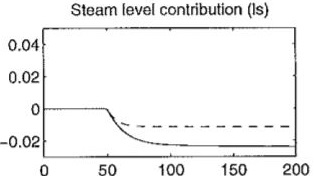
\includegraphics{Modeling/4State/AB_Figures/Figure8/Figure8-AB-5}}
                
                Figure 8 from \r{A}str\"{o}m and Bell's paper, section 5 \cite{Astrom}
                
                \resizebox{\ScaleMLFigThree \textwidth}{!}{\includegraphics{Modeling/4State/Matlab/Figure32/Figure32-5}}
                
                Simulation Results using Model from Eq \eqref{eq:Model_1}
                
                \caption{Steam Level Contribution to a step corresponding to 10 kg/s in feed water flow rate}
                \label{fig:Fig8C}
            \end{center}
        \end{figure}  % Level Steam Contribution    
        
        \begin{figure}[ht]
            \begin{center}
                \resizebox{\ScaleABFigThree \textwidth}{!}{\includegraphics{Modeling/4State/AB_Figures/Figure8/Figure8-AB-2}}
                
                Figure 8 from \r{A}str\"{o}m and Bell's paper, section 5 \cite{Astrom}
                
                \resizebox{\ScaleMLFigThree \textwidth}{!}{\includegraphics{Modeling/4State/Matlab/Figure32/Figure32-2}}
                
                Simulation Results using Model from Eq \eqref{eq:Model_1}
                
                \caption{Drum Pressure Response to a step corresponding to 10 kg/s in feed water flow rate}
                \label{fig:Fig8D}
            \end{center}
        \end{figure}  % Drum Pressure
        \begin{figure}[ht]
            \begin{center}
                \resizebox{\ScaleABFigThree \textwidth}{!}{\includegraphics{Modeling/4State/AB_Figures/Figure8/Figure8-AB-4}}
                
                Figure 8 from \r{A}str\"{o}m and Bell's paper, section 5 \cite{Astrom}
                
                \resizebox{\ScaleMLFigThree \textwidth}{!}{\includegraphics{Modeling/4State/Matlab/Figure32/Figure32-4}}
                
                Simulation Results using Model from Eq \eqref{eq:Model_1}
                
                \caption{Steam Volume Ratio Response to a step corresponding to 10 kg/s in feed water flow rate}
                \label{fig:Fig8E}
            \end{center}
        \end{figure}  % Steam Volume Ratio 
        \begin{figure}[ht]
            \begin{center}
                \resizebox{\ScaleABFigThree \textwidth}{!}{\includegraphics{Modeling/4State/AB_Figures/Figure8/Figure8-AB-6}}
                
                Figure 8 from \r{A}str\"{o}m and Bell's paper, section 5 \cite{Astrom}
                
                \resizebox{\ScaleMLFigThree \textwidth}{!}{\includegraphics{Modeling/4State/Matlab/Figure32/Figure32-6}}
                
                Simulation Results using Model from Eq \eqref{eq:Model_1}
                
                \caption{Steam Quality Response to a step corresponding to 10 kg/s in feed water flow rate}
                \label{fig:Fig8F}
                
            \end{center}
        \end{figure}  % Steam Quality
        
        10$^O$C Feed Water Step Responses: Figures \ref{fig:Fig9A}-\ref{fig:Fig9F}
        \begin{figure}[ht]
            \begin{center}
                \resizebox{\ScaleABFigThree \textwidth}{!}{\includegraphics{Modeling/4State/AB_Figures/Figure9/Figure9-AB-1}}
                
                Figure 9 from \r{A}str\"{o}m and Bell's paper, section 5 \cite{Astrom}
                
                \resizebox{\ScaleMLFigThree \textwidth}{!}{\includegraphics{Modeling/4State/Matlab/Figure42/Figure42-1}}
                
                Simulation Results using Model from Eq \eqref{eq:Model_1}
                
                \caption{Drum Water Level Response to a step corresponding to 10$^O$C Feed Water Temperature}
                \label{fig:Fig9A}
            \end{center}
        \end{figure}  % Level
        \begin{figure}[ht]
            \begin{center}
                \resizebox{\ScaleABFigThree \textwidth}{!}{\includegraphics{Modeling/4State/AB_Figures/Figure9/Figure9-AB-3}}
                
                Figure 9 from \r{A}str\"{o}m and Bell's paper, section 5 \cite{Astrom}
                
                \resizebox{\ScaleMLFigThree \textwidth}{!}{\includegraphics{Modeling/4State/Matlab/Figure42/Figure42-3}}
                
                Simulation Results using Model from Eq \eqref{eq:Model_1}
                
                \caption{Water Level Contribution to a step corresponding to 10$^O$C Feed Water Temperature}
                \label{fig:Fig9B}
            \end{center}
        \end{figure}  % Level Water Contribution
        \begin{figure}[ht]
            \begin{center}
                \resizebox{\ScaleABFigThree \textwidth}{!}{\includegraphics{Modeling/4State/AB_Figures/Figure9/Figure9-AB-5}}
                
                Figure 9 from \r{A}str\"{o}m and Bell's paper, section 5 \cite{Astrom}
                
                \resizebox{\ScaleMLFigThree \textwidth}{!}{\includegraphics{Modeling/4State/Matlab/Figure42/Figure42-5}}
                
                Simulation Results using Model from Eq \eqref{eq:Model_1}
                
                \caption{Steam Level Contribution to a step corresponding to 10$^O$C Feed Water Temperature}
                \label{fig:Fig9C}
            \end{center}
        \end{figure}  % Level Steam Contribution    
        
        \begin{figure}[ht]
            \begin{center}
                \resizebox{\ScaleABFigThree \textwidth}{!}{\includegraphics{Modeling/4State/AB_Figures/Figure9/Figure9-AB-2}}
                
                Figure 9 from \r{A}str\"{o}m and Bell's paper, section 5 \cite{Astrom}
                
                \resizebox{\ScaleMLFigThree \textwidth}{!}{\includegraphics{Modeling/4State/Matlab/Figure42/Figure42-2}}
                
                Simulation Results using Model from Eq \eqref{eq:Model_1}
                
                \caption{Drum Pressure Response to a step corresponding to 10$^O$C Feed Water Temperature}
                \label{fig:Fig9D}
            \end{center}
        \end{figure}  % Drum Pressure
        \begin{figure}[ht]
            \begin{center}
                \resizebox{\ScaleABFigThree \textwidth}{!}{\includegraphics{Modeling/4State/AB_Figures/Figure9/Figure9-AB-4}}
                
                Figure 9 from \r{A}str\"{o}m and Bell's paper, section 5 \cite{Astrom}
                
                \resizebox{\ScaleMLFigThree \textwidth}{!}{\includegraphics{Modeling/4State/Matlab/Figure42/Figure42-4}}
                
                Simulation Results using Model from Eq \eqref{eq:Model_1}
                
                \caption{Steam Volume Ratio Response to a step corresponding to 10$^O$C Feed Water Temperature}
                \label{fig:Fig9E}
            \end{center}
        \end{figure}  % Steam Volume Ratio 
        \begin{figure}[ht]
            \begin{center}
                \resizebox{\ScaleABFigThree \textwidth}{!}{\includegraphics{Modeling/4State/AB_Figures/Figure9/Figure9-AB-6}}
                
                Figure 9 from \r{A}str\"{o}m and Bell's paper, section 5 \cite{Astrom}
                
                \resizebox{\ScaleMLFigThree \textwidth}{!}{\includegraphics{Modeling/4State/Matlab/Figure42/Figure42-6}}
                
                Simulation Results using Model from Eq \eqref{eq:Model_1}
                
                \caption{Steam Quality Response to a step corresponding to 10$^O$C Feed Water Temperature}
                \label{fig:Fig9F}
            \end{center}
        \end{figure}  % Steam Quality
        
        \clearpage
        
        Using Figures \ref{fig:Fig6A} - \ref{fig:Fig4D} to compare the shape and scale of the graphed outputs from the simulated model and the corresponding output from the \r{A}str\"{o}m and Bell paper, it can be concluded that for a 10 MW fuel flow step increase, the system responses behave similarly. While the specific values may not match exactly due to a difference in calculated Initial Conditions, the same trends are shown on all of the curves. 
        \begin{rem}
            For $u(3) = Q$ the simulated model \eqref{eq:Model_1} has the same step response as the \r{A}str\"{o}m and Bell model
            \label{remark:u3}
        \end{rem}
        
        Using Figures \ref{fig:Fig7A} - \ref{fig:Fig5D} to compare the shape and scale of the graphed outputs from the simulated model and the corresponding output from the \r{A}str\"{o}m and Bell paper, it can be concluded that for a 10 kg/s in steam flow step increase, the system responses behave similarly. While the specific values may not match exactly due to a difference in calculated Initial Conditions, the same trends are shown on all of the curves. 
        \begin{rem}
            For $u(2) = q_s$ the simulated model \eqref{eq:Model_1} has the same step response as the \r{A}str\"{o}m and Bell model
            \label{remark:u2}
        \end{rem}
        
        Using Figures \ref{fig:Fig8A} - \ref{fig:Fig8F} to compare the shape and scale of the graphed outputs from the simulated model and the corresponding output from the \r{A}str\"{o}m and Bell paper, it can be concluded that for a  10 kg/s in feed water flow step increase, the system responses behave similarly. While the specific values may not match exactly due to a difference in calculated Initial Conditions, the same trends are shown on all of the curves. 
        \begin{rem}
            For $u(1) = q_f$ the simulated model \eqref{eq:Model_1} has the same step response as the \r{A}str\"{o}m and Bell model
            \label{remark:u1}
        \end{rem}
        
        Using Figures \ref{fig:Fig9A} - \ref{fig:Fig9F} to compare the shape and scale of the graphed outputs from the simulated model and the corresponding output from the \r{A}str\"{o}m and Bell paper, it can be concluded that for a 10$^O$C Feed Water temperature step  increase, the system responses behave similarly. While the specific values may not match exactly due to a difference in calculated Initial Conditions, the same trends are shown on all of the curves. 
        \begin{rem}
            For $u(4) = t_f$ the simulated model \eqref{eq:Model_1} has the same step response as the \r{A}str\"{o}m and Bell model
            \label{remark:u4}
        \end{rem}
        
        If Remarks \ref{remark:u3} - \ref{remark:u4} are true, and all of the inputs to the model \eqref{eq:Model_1} have been tested then at the specified initial conditions it can be concluded that the model matches the \r{A}str\"{o}m and Bell model.
        
\section{Expanded Model}
    
    The \r{A}str\"{o}m and Bell model uses 4 inputs, $q_f$, $q_s$, $Q$, $t_f$. Expansion upon this allows for a simpler control design. Basic assumptions and methods from previous works allow for the inputs to be lowered down to 2. 
    
    \subsection{Input Simplifications}
    
        \subsubsection{Feedwater}
            Feed-water temperature can usually be considered constant. Once an equilibrium value is found, this can reduce the number of inputs into the model. 
            
            $$ t_{f} = t_{f0} = constant$$
            
            This constant is then used to simplify the inputs from 4 to 3. 
            
        \subsubsection{Steam Flow}
            Steam flow ($q_s$) can be converted from an input to the model if the throttle pressure and throttle valve are modeled. \cite{Iacob}
            
            $$ \aligned
                p - p_t =&K_{sh} \left ( \frac{ q_s}{k_v} \right )^{2} \\
                q_s =& \mu p_t 
            \endaligned$$
            
            $K_v$ becomes a new input from 0-1, which is the throttle valve coefficient. 
            
            Throttle Pressure can be estimated as being between 5\% and 10\% of the drum pressure.\cite{IacobEmail} $K_{sh}$ and $\mu$ can be determined using this information and the above equations. For all simulations, the throttle valve will be left full open, to reduce the number of inputs again. 
            
            $$ \aligned
                K_{sh} =& 0.0013  \\
                \mu    =& 6.77 \\ 
                k_v    =& 1
            \endaligned$$
                

            This then produces: 
            
            $$p  = K_{sh} q_s^{2} + \frac{ q_s}{\mu} \Longrightarrow  q_s = f(p)$$
            %$$\frac { \sqrt{ K_{sh} p \mu^2 4+1} - 1 } {2 K_{sh} \mu}$$
            
            This function further simplifies the inputs from 3 (see Feedwater above) to 2, as $q_s$ is now a direct function of $p$. 
            
        \subsubsection{Valve Dynamics}
            The remaining inputs are controlled by valves, so first order approximations for the valve movement was added. In the below, $T_{v_{Q }}$ and $T_{v_{fw}}$ are the valve time constants.  
            
            $$ \dot{Q}_{valve}  = \frac{\left(  Q_{valve}  - Q       \right)}{T_{v_{Q }}}$$
            $$ \dot{FW}_{valve} = \frac{\left( FW_{valve}  - q_{fw}  \right)}{T_{v_{fw}}}$$
            
            This can be put into matrix form to in the following way:
            \begin{equation}
                \frac{\mathrm{d} }{\mathrm{d} t} 
                \left [ \begin{matrix} Q_{valve} \\ FW_{valve} \end{matrix} \right ]  
                =
                \left[ \begin{matrix} \frac{\left(  Q_{valve}  - Q       \right)}{T_{v_{Q }}} \\\frac{\left( FW_{valve}  - q_{fw}  \right)}{T_{v_{fw}}}   \end{matrix} \right]
                \label{eq:Valve_model_A}
            \end{equation}
            These were then incorporated into the state equation, creating a 6 function nonlinear differential equation, with 6 states and 2 inputs. 
            
            $$ \begin{matrix} V_{wt} & p& \alpha_r& V_{sd} & Q & q_{fw}\end{matrix} $$
            $$ \begin{matrix} Q_{valve} & FW_{valve} \end{matrix} $$
        
    \subsection{Expanded Model with Simplified Inputs}
        Combining Equations \ref{eq:Model_1} and \ref{eq:Valve_model_A} results in the following:
        \begin{equation}
            \label{eq:Valve_Model_1}
            \frac{\mathrm{d} }{\mathrm{d} t} 
            \left [ \begin{matrix} \left [ \begin{matrix} V_{wt}\\ p\\ \alpha_r\\ V_{sd}\end{matrix} \right ]  \\ \left [ \begin{matrix} Q_{valve} \\ FW_{valve} \end{matrix} \right ] \end{matrix} \right ]  
            =
            \left [ \begin{matrix}  \left [ \begin{matrix}e_{11}& e_{12}& 0& 0 \\ e_{21}& e_{22}& 0& 0 \\ 0 & e_{32}& e_{33}& 0 \\ 0 & e_{42}& e_{43}& e_{44}\end{matrix} \right ] ^{-1} \left [ \begin{matrix} q_f  - q_s \\ Q + q_f h_f  - q_s h_s\\ Q + \alpha_r h_c q_{dc} \\ \frac{\rho_s}{T_d}  \left ( V_{sd}^0  - V_{sd}\right ) + \frac{h_f - h_w}{h_c}q_f \end{matrix} 
            \right ] \\  \left[ \begin{matrix} \frac{\left(  Q_{valve}  - Q       \right)}{T_{v_{Q }}} \\\frac{\left( FW_{valve}  - q_{fw}  \right)}{T_{v_{fw}}}   \end{matrix} \right]  \end{matrix} \right ]
        \end{equation}
     
        It should be noted that Equation \ref{eq:Valve_Model_1} is in terms of
        $$ \dot{x} = f\left (x, u\right)$$
        Where:
        $$ x = \left [\begin{matrix} V_{wt} & p & \alpha_r & V_{sd} & Q & q_{fw}\end{matrix} \right]^T$$
        $$ u = \left [\begin{matrix} Q_{valve} & FW_{valve} \end{matrix} \right]^T$$        
        
        This is the form of a Nonlinear-Time-Invariant State Space system. 
        
        A list of simplifications made for the final model used \eqref{eq:Valve_Model_1} are as follows:
    
        \begin{itemize}
          \item Feed water Valve is treated as a first order system compared to Feed water Flow
          \item Fuel Valve is treated as a first order system compared to Heat transfer into the boiler. This is an oversimplification of the fuel flow dynamics, which consist of fuel flow and air flow. Air flow is normally controlled by excess flue oxygen and the stoichiometric ratio to fuel flow.  
          \item Feed water Temperature is treated as constant
          \item Steam Flow is estimated based off of throttle pressure
          \item Properties of water are modeled based off of numerical evidence
        \end{itemize}        
    
    \subsection{Open Loop Step Responses to Expanded Model}
    
        The model used in Eq. \ref{eq:Valve_Model_1} was simulated with step inputs, the results are the following figures. 
        
        Figures \ref{fig:Valve_Open1A} - \ref{fig:Valve_Open1E} use the model \eqref{eq:Valve_Model_1}, while Figures \ref{fig:Fig6A} - \ref{fig:Fig6F} uses the model \eqref{eq:Model_1}. Both sets of figures use the same step input of $Q$ = 10 MW, however the expanded model uses a first order dynamic delay. 
        
        Figures \ref{fig:Valve_Open2A} - \ref{fig:Valve_Open2E} use the model \eqref{eq:Valve_Model_1}, while Figures \ref{fig:Fig8A} - \ref{fig:Fig8F} uses the model \eqref{eq:Model_1}. Both sets of figures use the same step input of $q_f$ = 10 kg/s, however the expanded model uses a first order dynamic delay. 
        
        \begin{figure}[ht]
            \begin{center}
                \resizebox{\ScaleMLFigThree \textwidth}{!}{\includegraphics{Modeling/6State/Matlab/Figure81/Figure81-1}}
                
                Short Term Step Response
                
                \resizebox{\ScaleMLFigThree \textwidth}{!}{\includegraphics{Modeling/6State/Matlab/Figure82/Figure82-1}}
                
                Long Term Step Response
                
                \caption{Drum Water Level Response to a step corresponding to 10 MW in fuel flow rate}
                \label{fig:Valve_Open1A}
            \end{center}
            Figure \ref{fig:Valve_Open1A} should be directly compared to Figure \ref{fig:Fig6A}. This shows the shrink/swell effect, in how level initially reacts in one direction, however it ultimately trends towards the opposite direction.
        \end{figure}  % A Level
        
        
        \begin{figure}[ht]
            \begin{center}
                \resizebox{\ScaleMLFigThree \textwidth}{!}{\includegraphics{Modeling/6State/Matlab/Figure81/Figure81-2}}
                
                Short Term Step Response
                
                \resizebox{\ScaleMLFigThree \textwidth}{!}{\includegraphics{Modeling/6State/Matlab/Figure82/Figure82-2}}
                
                Long Term Step Response
                
                \caption{Drum Pressure Response to a step corresponding to 10 MW in fuel flow rate}
                \label{fig:Valve_Open1B}
            \end{center}
            Figure \ref{fig:Valve_Open1B} should be directly compared to Figure \ref{fig:Fig6D}, the initial response matches what was seen in the \r{A}str\"{o}m and Bell paper and pressure eventually reaches a stable settling point.
        \end{figure}  % B Pressure  
        
        \begin{figure}[ht]
            \begin{center}
                \resizebox{\ScaleMLFigThree \textwidth}{!}{\includegraphics{Modeling/6State/Matlab/Figure81/Figure81-3}}
                
                Short Term Step Response
                
                \resizebox{\ScaleMLFigThree \textwidth}{!}{\includegraphics{Modeling/6State/Matlab/Figure82/Figure82-3}}
                
                Long Term Step Response
                
                \caption{Volume of Total Water Response to a step corresponding to 10 MW in fuel flow rate}
                \label{fig:Valve_Open1C}
            \end{center}
            Figure \ref{fig:Valve_Open1C} is not directly comparable to a figure from the \r{A}str\"{o}m and Bell paper, however it makes sense that if the feed water valve is held constant but more heat is added that water will eventually leave the system in the form of steam. 
        \end{figure}  % C Volume of Water Total
        
        \begin{figure}[ht]
            \begin{center}
                \resizebox{\ScaleMLFigThree \textwidth}{!}{\includegraphics{Modeling/6State/Matlab/Figure81/Figure81-4}}
                
                Short Term Step Response
                
                \resizebox{\ScaleMLFigThree \textwidth}{!}{\includegraphics{Modeling/6State/Matlab/Figure82/Figure82-4}}
                
                Long Term Step Response
                
                \caption{Steam Quality Response to a step corresponding to 10 MW in fuel flow rate}
                \label{fig:Valve_Open1D}
            \end{center}
            Figure \ref{fig:Valve_Open1D} should be directly compared to Figure \ref{fig:Fig6F}, the initial response matches what was seen in the \r{A}str\"{o}m and Bell paper and steam quality eventually reaches a stable settling point.
        \end{figure}  % D Steam Quality 
        
        \begin{figure}[ht]
            \begin{center}
                \resizebox{\ScaleMLFigThree \textwidth}{!}{\includegraphics{Modeling/6State/Matlab/Figure81/Figure81-5}}
                
                Short Term Step Response
                
                \resizebox{\ScaleMLFigThree \textwidth}{!}{\includegraphics{Modeling/6State/Matlab/Figure82/Figure82-5}}
                
                Long Term Step Response
                
                \caption{Volume of Steam in the Drum Response to a step corresponding to 10 MW in fuel flow rate}
                \label{fig:Valve_Open1E}
            \end{center}
            Figure \ref{fig:Valve_Open1E} should be directly compared to Figure \ref{fig:Fig6C}, as the volume of steam in the drum is directly proportional to the steam level contribution. As seen in the level plots (Figure \ref{fig:Valve_Open1A}) the shirnk/swell effect can be partially seen here. 
        \end{figure}  % E Volume of Steam Drum     
        
        \begin{figure}[ht]
            \begin{center}
                \resizebox{\ScaleMLFigThree \textwidth}{!}{\includegraphics{Modeling/6State/Matlab/Figure91/Figure91-1}}
                
                Short Term Step Response
                
                \resizebox{\ScaleMLFigThree \textwidth}{!}{\includegraphics{Modeling/6State/Matlab/Figure92/Figure92-1}}
                
                Long Term Step Response
                
                \caption{Drum Water Level Response to a step corresponding to 10 kg/s feed water flow rate}
                \label{fig:Valve_Open2A}
            \end{center}
            Figure \ref{fig:Valve_Open2A} should be directly compared to Figure \ref{fig:Fig8A}. This shows the shrink/swell effect, in how level initially reacts in one direction, however it ultimately trends towards the opposite direction.
        \end{figure}  % A Level
        
        \begin{figure}[ht]
            \begin{center}
                \resizebox{\ScaleMLFigThree \textwidth}{!}{\includegraphics{Modeling/6State/Matlab/Figure91/Figure91-2}}
                
                Short Term Step Response
                
                \resizebox{\ScaleMLFigThree \textwidth}{!}{\includegraphics{Modeling/6State/Matlab/Figure92/Figure92-2}}
                
                Long Term Step Response
                
                \caption{Drum Pressure Response to a step corresponding to 10 kg/s feed water flow rate}
                \label{fig:Valve_Open2B}
            \end{center}
            Figure \ref{fig:Valve_Open2B} should be directly compared to Figure \ref{fig:Fig8D}, the initial response matches what was seen in the \r{A}str\"{o}m and Bell paper and pressure eventually reaches a stable settling point.
        \end{figure}  % B Pressure 
        
        \begin{figure}[ht]
            \begin{center}
                \resizebox{\ScaleMLFigThree \textwidth}{!}{\includegraphics{Modeling/6State/Matlab/Figure91/Figure91-3}}
                
                Short Term Step Response
                
                \resizebox{\ScaleMLFigThree \textwidth}{!}{\includegraphics{Modeling/6State/Matlab/Figure92/Figure92-3}}
                
                Long Term Step Response
                
                \caption{Volume of Total Water Response to a step corresponding to 10 kg/s feed water flow rate}
                \label{fig:Valve_Open2C}
            \end{center}
            Figure \ref{fig:Valve_Open2C} is not directly comparable to a figure from the \r{A}str\"{o}m and Bell paper, however it makes sense that if the feed water increased from a stable operating point and all other inputs are held constant, then more water will eventually fill the drum. 
        \end{figure}  % C Volume of Water Total
        
        \begin{figure}[ht]
            \begin{center}
                \resizebox{\ScaleMLFigThree \textwidth}{!}{\includegraphics{Modeling/6State/Matlab/Figure91/Figure91-4}}
                
                Short Term Step Response
                
                \resizebox{\ScaleMLFigThree \textwidth}{!}{\includegraphics{Modeling/6State/Matlab/Figure92/Figure92-4}}
                
                Long Term Step Response
                
                \caption{Steam Quality Response to a step corresponding to 10 kg/s feed water flow rate}
                \label{fig:Valve_Open2D}
            \end{center}
            Figure \ref{fig:Valve_Open2D} should be directly compared to Figure \ref{fig:Fig8F}, the initial response matches what was seen in the \r{A}str\"{o}m and Bell paper and steam quality eventually reaches a stable settling point.
        \end{figure}  % D Steam Quality 
        
        \begin{figure}[ht]
            \begin{center}
                \resizebox{\ScaleMLFigThree \textwidth}{!}{\includegraphics{Modeling/6State/Matlab/Figure91/Figure91-5}}
               
                Short Term Step Response
                
                \resizebox{\ScaleMLFigThree \textwidth}{!}{\includegraphics{Modeling/6State/Matlab/Figure92/Figure92-5}}
                
                Long Term Step Response
                
                \caption{Volume of Steam in the Drum Response to a step corresponding to 10 kg/s feed water flow rate}
                \label{fig:Valve_Open2E}
            \end{center}
            Figure \ref{fig:Valve_Open2E} should be directly compared to Figure \ref{fig:Fig8C}, as the volume of steam in the drum is directly proportional to the steam level contribution. 
        \end{figure}  % E Volume of Steam Drum  
        
        

        \clearpage
        %What can be seen in Figure \ref{fig:Valve_Open1B} and \ref{fig:Valve_Open2B} are the long term responses of step inputs of Megawatts (in terms of heat input) and feed water flow. Figure \ref{fig:Valve_Open1B} shows expected values eventually becoming stable, such as drum pressure. What is worth noting though is the early dynamics, which can be see in in Figure \ref{fig:Valve_Open1A} and in particular the drum water level behaves in direct opposition to how it behaves in the long term. Initially the drum water rises, sees some effects of shrink/swell, but overall rises. The long term response though shows drum level as near constantly decreasing. Figure\ref{fig:Valve_Open2B} shows expected values eventually becoming stable, and drum level constantly rising, which is to be expected if water is constantly added into the drum. The early responses are also acting differently to the overall trend, but to a lesser extent.
        
        These simulations do not take into account that the drum has a completely finite volume to fill nor does it take into account the possibility of bursting from high pressure. Future work could expand upon this, however this is not necessary for this paper. The goal of these long term simulations was to determine that the shrink/swell effect was occurring and on what timescale would it be necessary to see those effects. Future simulations will be well within physical controllable ranges. 

    \chapter{Three Element Control}

As discussed in Section 2.1, PID control is by design not optimized. It is however a proven tool used in industry and has been able to satisfactorily control boilers for decades. This chapter will discuss on the physical dynamics of how the PID control strategy seen in Figure \ref{fig:3_element_control} can be used on the Expanded model in Equation \ref{eq:Valve_Model_1} without linearization. It should be noted that many power plants use adaptive controller gains in conjecture with the three element control stragety. 

   %     $$ x = \left [\begin{matrix} V_{wt} & p & \alpha_r & V_{sd} & Q & q_{fw}\end{matrix} \right]^T$$
   %     $$ u = \left [\begin{matrix}  & FW_{valve} \end{matrix} \right]^T$$  

\section{Controller Design}

    The model in place requires control inputs to the Feed Water Valve and the Fuel Valve. The Fuel valve controls pressure directly, but due to the dynamics of the boiler, level control cannot be decoupled entirely, and the steam flow out becomes part of the three element controller. 
    
    For this design, the Controlers were tuned to be stable, but not optimized. 
    
    The controller for the Pressure is designed as a PI controller with the following gains:
    $$ \begin{matrix} K_p = 100   & & & K_i = 0.15 \end{matrix} $$
    \begin{equation}
        \label{eq:PID_Q_VALVE}
        Q_{valve} = \left( K_p + K_i \frac{1}{s} \right)\left( p_{ref} - p \right)
    \end{equation}
    The Three Element controller follows the format shown in Figure \ref{fig:Alt_3_element_control}. 
    
    The Level Controller has the following Gains:
    $$ \begin{matrix} K_p = 250   & & & K_i = 1 \end{matrix} $$
    \begin{equation}
        \label{eq:PID_FW_SP}
        q_{fw sp} = \left( K_p + K_i \frac{1}{s} \right)\left( l_{ref} - l \right)
    \end{equation}
    
    The Level Controller then feeds into the Feed Water Controller and the Feed Water Controller has a feed Forward. The following gains and equations apply:
    $$ \begin{matrix} K_p = 1 & & & K_i = 1  & & & K_{ff} = 1\end{matrix}$$
    \begin{equation}
        \label{eq:PID_FW_VALVE_1}
        FW_{valve} = \left( K_p + K_i \frac{1}{s} \right)\left( q_{fwsp} - q_{fw} \right) + K_{ff} q_s
    \end{equation}
    
    The cascaded control is then calculated by combining \eqref{eq:PID_FW_SP} and \eqref{eq:PID_FW_VALVE_1} to get \eqref{eq:PID_FW_VALVE}
    \begin{equation}
        \label{eq:PID_FW_VALVE}
        FW_{valve} = \left( K_p + K_i \frac{1}{s} \right)\left( \left( K_p + K_i \frac{1}{s} \right)\left( l_{ref} - l \right) - q_{fw} \right) + K_{ff} q_s
    \end{equation}
    
    These PID Controllers \eqref{eq:PID_Q_VALVE}\eqref{eq:PID_FW_VALVE} were integrated into the Expanded Valve Model seen in Equation \ref{eq:Valve_Model_1}, which increased the number of states by 3 (one for each I term in the PI Controllers). 
    The new state variable for the PID closed loop system is as follows:
    $$\begin{matrix} \left [ \begin{matrix} V_{wt} & p & \alpha_r & V_{sd} & Q_{valve} & FW_{valve} & \left( p_{ref} - p \right) & \left( q_{fwsp} - q_{fw} \right) & \left( l_{ref} - l \right) \end{matrix} \right ]^T \end{matrix}$$

\section{Simulation Results}

    The simulation using the PID can be calculated using the full nonlinear model, with no linearisation required. It should be noted that the chosen gain values may not control properly over a large range. 
    
    Below are Step Responses for changes in the Reference (Set Point) for the Drum Pressure Controller \eqref{eq:PID_Q_VALVE}.
    
    \begin{figure}[ht]
        \begin{center}
            \resizebox{\ScaleMLFigFour \textwidth}{!}{\includegraphics{Controlers/ThreeElement/PressStep/PID1/PID1-3.jpg}}
            \caption{Drum Pressure PID Response to Drum Pressure increase of 0.1}
            \label{fig:PID_Pressure_PressStep}
        \end{center}
    \end{figure}  % Drum Pressure PID     Response to Drum Pressure increase of 0.1  
    \begin{figure}[ht]
        \begin{center}
            \resizebox{\ScaleMLFigFour \textwidth}{!}{\includegraphics{Controlers/ThreeElement/PressStep/PID1/PID1-6.jpg}}
            \caption{Drum Pressure Control Response $Q_{valve}$ to Drum Pressure increase of 0.1}
            \label{fig:PID_Pressure_PressStep_Control}
        \end{center}
    \end{figure}  % Drum Pressure Control Response to Drum Pressure increase of 0.1     
    
    \begin{figure}[ht]
        \begin{center}
            \resizebox{\ScaleMLFigFour \textwidth}{!}{\includegraphics{Controlers/ThreeElement/LvlStep/PID4/PID4-3.jpg}}
            \caption{Drum Pressure PID Response to Level increase of 0.1}
            \label{fig:PID_Pressure_LvlStep}
        \end{center}
    \end{figure}  % Drum Pressure PID Response to Level increase of 0.1    
    \begin{figure}[ht]
        \begin{center}
            \resizebox{\ScaleMLFigFour \textwidth}{!}{\includegraphics{Controlers/ThreeElement/LvlStep/PID4/PID4-6.jpg}}
            \caption{Drum Pressure Control Response $Q_{valve}$ to Level increase of 0.1}
            \label{fig:PID_Pressure_LvlStep_Control}
        \end{center}
    \end{figure}  % Drum Pressure Control Response to Level increase of 0.1   
    
    Figures \ref{fig:PID_Pressure_PressStep}-\ref{fig:PID_Pressure_LvlStep_Control} show that the model chosen can have pressure adequately controlled by a simple PID. In figure \ref{fig:PID_Pressure_PressStep_Control} it should be noted that a drastic jump in the control is used. This is to be considered heat demand, as $Q_{valve}$ is a simplification of heat addition into the boiler, and the state $Q$ does not have such a drastic curve. Figures \ref{fig:PID_Pressure_PressStep}-\ref{fig:PID_Pressure_PressStep_Control} shows a step response with desirable control settings. Figures \ref{fig:PID_Pressure_LvlStep}-\ref{fig:PID_Pressure_LvlStep_Control} shows a disturbance rejection, as the set point for Drum Pressure never changes. The initial response and long settling time appear as if they can be improved upon.
    
    %% NOTE TO SELF BORZELLIERI BISWAS Search tag: Add in graph for Q vs Q_valve. Reprint PIDs so that it doesn't say Steam valve. That is wrong. 
    
    \clearpage
    
    Below are the Step Responses for the changes in Reference (Set Point) for the \textit{Three Element} Level Controller.
    
    \begin{figure}[ht]
        \begin{center}
            \resizebox{\ScaleMLFigFour \textwidth}{!}{\includegraphics{Controlers/ThreeElement/PressStep/PID1/PID1-2.jpg}}
            \caption{Drum Level PID Response to Drum Pressure increase of 0.1}
            \label{fig:PID_Level_PressStep}
        \end{center}
    \end{figure}   % Drum Level PID Response to  Drum Pressure increase of 0.1
    \begin{figure}[ht]
        \begin{center}
            \resizebox{\ScaleMLFigFour \textwidth}{!}{\includegraphics{Controlers/ThreeElement/PressStep/PID1/PID1-1.jpg}}
            \caption{Feedwater PID Response to Cascaded Control Set Point}
            \label{fig:PID_Feedwater_PressStep}
        \end{center}
    \end{figure}   % Feedwater PID Response to Cascaded Control Set Point
    \begin{figure}[ht]
        \begin{center}
            \resizebox{\ScaleMLFigFour \textwidth}{!}{\includegraphics{Controlers/ThreeElement/PressStep/PID1/PID1-4.jpg}}
            \caption{Feedwater Valve and Steam Flow (Feed Forward) to Feedwater Cascaded Control}
            \label{fig:PID_Feedwater_PressStep_Control}    
        \end{center}
    \end{figure}   % Feedwater Valve and Steam Flow (Feed Forward) to Feedwater Cascaded Control
    
    \begin{figure}[ht]
        \begin{center}
            \resizebox{\ScaleMLFigFour \textwidth}{!}{\includegraphics{Controlers/ThreeElement/LvlStep/PID4/PID4-2.jpg}}
            \caption{Drum Level PID Response to a Level increase of 0.1}
            \label{fig:PID_Level_LvlStep}
        \end{center}
    \end{figure}   % Drum Level PID Response to a Level increase of 0.1
    \begin{figure}[ht]
        \begin{center}
            \resizebox{\ScaleMLFigFour \textwidth}{!}{\includegraphics{Controlers/ThreeElement/LvlStep/PID4/PID4-1.jpg}}
            \caption{Feedwater PID Response to Cascaded Control Set Point}
            \label{fig:PID_Feedwater_LvlStep}
        \end{center}
    \end{figure}   % Feedwater PID Response to Cascaded Control Set Point
    \begin{figure}[ht]
        \begin{center}
            \resizebox{\ScaleMLFigFour \textwidth}{!}{\includegraphics{Controlers/ThreeElement/LvlStep/PID4/PID4-4.jpg}}
            \caption{Feedwater Valve and Steam Flow (Feed Forward) to Feedwater Cascaded Control}
            \label{fig:PID_Feedwater_LvlStep_Control} 
        \end{center}
    \end{figure}   % Feedwater Valve and Steam Flow (Feed Forward) to Feedwater Cascaded Control
    
    Figures \ref{fig:PID_Level_PressStep}-\ref{fig:PID_Feedwater_LvlStep_Control} show that the model chosen can have drum level adequately controlled by the three element control strategy used in industry. Figures \ref{fig:PID_Level_LvlStep}-\ref{fig:PID_Feedwater_LvlStep_Control} shows a step response in terms of level, as the Drum Level set point increases by 0.1. Note the inner loop of Feedwater Flow has its set point change drastically to maintain level. Figures \ref{fig:PID_Level_PressStep}-\ref{fig:PID_Feedwater_PressStep_Control} shows a disturbance response in terms of level, as the Drum Level set point stays constant. Note the inner loop of Feedwater Flow has its set point change drastically to maintain level. Figures \ref{fig:PID_Level_PressStep} \& \ref{fig:PID_Level_LvlStep} show the controller output for the level controller. The controller output for these loops is a set point for the inner cascade loop, and can be see on figures \ref{fig:PID_Feedwater_PressStep} \& \ref{fig:PID_Feedwater_PressStep_Control}. Figures \ref{fig:PID_Feedwater_PressStep} \& \ref{fig:PID_Feedwater_LvlStep} show the tracking response of the inner cascade controller for Feedwater, and Figures \ref{fig:PID_Feedwater_PressStep_Control} \& \ref{fig:PID_Feedwater_LvlStep_Control} show the controller output. Figures \ref{fig:PID_Feedwater_PressStep_Control} \& \ref{fig:PID_Feedwater_LvlStep_Control} also show steam flow, as it is a feed forward to the controller. 
    
    %% NOTE TO SELF BORZELLIERI BISWAS (Search tags): Update Graphics to show Feedwater Valve and Steam Flow, and Feedwater SP vs Feedwater Flow. 
    \chapter{Future Work}

The goals of this paper are to investigate the limitations of conventional controls systems, and analyze if a more complex approach, such as MPC. A boiler model has been created \eqref{eq:Valve_Model_1} and verified against previous work, and {\it three element control} has been simulated. Future work includes controller design for both LQR and MPC, as well as an analysis of the controllers. 

\section{Linear Quadratic Regulator}

    Citing previous works, the plant will be linearized at 50\% of full load and then a LQR controller will be designed by adopting a cheap control methodology and using trial and error methods. This linearly designed controller will then be applied to the nonlinear system \eqref{eq:Valve_Model_1}.

\section{Model Predictive Control}

    Using the model \eqref{eq:Valve_Model_1}, the algorithm \ref{algorithm:NonLinMPC} will be applied as a nonlinear controller. Design considerations will be made for $N_p$ and $N_c$, as they will be critical in the control implication. If too small, the shrink/swell effects will drive the calculations and cause instability. If too large, calculation times will exceed what is practical for use. 

\section{Analysis}

    A controller analysis will be created comparing the Settling Time and Overshoot (\%) for all three controllers. A similar analysis was done in previous works \cite{Panwar}, however that comparison was between controllers that used a Steam Turbine Valve and a Feed Water Valve as inputs and treated Heat input as a disturbance. Figure 14-15 and Table 3 in \cite{Panwar} compare the different controllers and a similar analysis will be performed here, however control input will also be considered. 
    %\chapter{LQR Controller Design}

\section{LQR methods}

Dummy Text
plant linearized at 50\% of full power(FP) \cite{Panwar}

Selecting Q and R matrices is a crucial step in LQR
design. Adopting cheap control methodology [11] and using
trial and error method, the values for Q and R matrix are
selected as follows

    %\chapter{Design of Model Predictive Controller}

\section{Self Notes}
        \clearpage
        
        The system:
        
        \begin{equation*}
            \frac{\mathrm{d} }{\mathrm{d} t} 
            \left [ \begin{matrix}  V_{wt}\\ p\\ \alpha_r\\ V_{sd} \\  Q_{valve} \\ FW_{valve}  \end{matrix} \right ]  
            =
            \left [ \begin{matrix}  \left [ \begin{matrix}e_{11}& e_{12}& 0& 0 \\ e_{21}& e_{22}& 0& 0 \\ 0 & e_{32}& e_{33}& 0 \\ 0 & e_{42}& e_{43}& e_{44}\end{matrix} \right ] ^{-1} \left [ \begin{matrix} q_f  - q_s \\ Q + q_f h_f  - q_s h_s\\ Q + \alpha_r h_c q_{dc} \\ \frac{\rho_s}{T_d}  \left ( V_{sd}^0  - V_{sd}\right ) + \frac{h_f - h_w}{h_c}q_f \end{matrix} 
            \right ] \\   \begin{matrix} \frac{\left(  Q_{valve}  - Q       \right)}{T_{v_{Q }}} \\\frac{\left( FW_{valve}  - q_{fw}  \right)}{T_{v_{fw}}}   \end{matrix}  \end{matrix} \right ]
        \end{equation*}
        
        A stable operating point was found to be:
        $$\begin{matrix}
            x\left (0 \right) = x_0 =   \left [\begin{matrix} V_{wt0}\\ p_{0}\\  \alpha_{r0}\\ V_{sd0}\\ Q_{0}\\ q_{fw}\end{matrix} \right ] = \left [ \begin{matrix} 57.1 \\ 8.5 \\ 0.0524 \\ 4.9 \\ 86.78 \\ 50.8 \end{matrix} \right ]
            & & 
            u\left (0 \right) =  u_0 = \left [\begin{matrix} Q_{valve0} \\ q_{valve0} \\ \end{matrix} \right ] =  \left [\begin{matrix} 86.78\\ 50.8 \\ \end{matrix} \right ]  
        \end{matrix}$$  
        
        \clearpage
        Can be considered a non-linear state space equation of the form:
        $$\dot{x}(t) = f\left ( x(t),u(t) \right )$$
        $$y(t) = g\left ( x(t),u(t) \right )$$
        
        This is then discretized, where $n$ is an integer, and $T$ is the sampling time. 
        
        $$ \begin{matrix} x(t) = x(nT) & & u(t) = u(nT) \end{matrix}$$
        
        This can be linearized around an operating point to create a state space model:
        $$ \begin{matrix} x(nT) & & u(nT) \end{matrix}$$
        $$\begin{matrix}
           \frac{\partial\Delta x(t)}{dt} = A_i^c \Delta x(t) + B_i^c \Delta u(t) & & &  A_i^c = \biggl.\frac{\partial f(x,u)}{\partial x}\biggr|_{x(nT), u(nT)} & & C_i^c = \biggl.\frac{\partial g(x,u)}{\partial x}\biggr|_{x(nT), u(nT)}\\
            \Delta y(t) = C_i^c \Delta x(t) + D_i^c \Delta u(t) & & & B_i^c = \biggl.\frac{\partial f(x,u)}{\partial u}\biggr|_{x(nT), u(nT)} & & D_i^c = \biggl.\frac{\partial g(x,u)}{\partial u}\biggr|_{x(nT), u(nT)}
        \end{matrix}$$
        It should be noted that:
        $$ \begin{matrix} x(t) = \Delta x(t) + x(nT) & & u(t) = \Delta u(t) + u(nT) \end{matrix}$$

        
        $$\begin{matrix}
            \Delta x(k_i+1) = A_i \Delta  x(k_i) + B_i \Delta  u(k_i) & & & A_i = e^{A_i^c T} & B_i = \left (  \int_{0}^{T} e^{A_i^c \tau}\, d\tau \right ) B_i^c \\
            \Delta y(k_i)   = C_i \Delta x(k_i) + D_i \Delta u(k_i)   & & & C_i = C_i^c       & D_i = D_i^c
        \end{matrix}$$

        $$K_{y_i} = \overset{N_c}{\overbrace{\begin{bmatrix} I& 0 & ... & 0 \end{bmatrix}}} (\Phi_i^{T}Q\Phi_i + R)^{-1}\Phi^{T}_i Q\overline{R_{s_i}}$$
        
        $$K_{mpc_i} = \overset{N_c}{\overbrace{\begin{bmatrix} I& 0 & ... & 0 \end{bmatrix}}} (\Phi_i^{T}Q\Phi_i + R)^{-1}\Phi^{T}_i Q F_i$$

        Where: 
        \begin{equation*}
           \aligned
                F_{i}^T &= \overset{N_p}{\overbrace{\begin{bmatrix} C_i A_i & C_i A^{2}_i & \cdots & C_i A^{N_{p}}_i \end{bmatrix}}} \\
                \Phi_i &=  \overset{N_c}{\overbrace{\left [ \begin{array}{ccccc}
                         C_i B_i & 0 & 0 & \cdots & 0 \\
                         C_i A_i B_i & C_i B_i & 0 & \cdots & 0 \\
                         C_i A^{2}_i B_i & C_i A_i B_i & C_i B_i & \cdots & 0 \\
                         \vdots & \vdots & \vdots & \ddots & \vdots \\
                         C_i A^{N_{p}-1}_i B_i & C_i A^{N_{p}-2}_i B_i & C_i A^{N_{p}-3}_i B_i & \cdots &  C_i A_{i}^{N_{p}-N_{c}} B_i \end{array}  \right ]}} \\
                \overline R_{s_i}^T &= \overset{N_p}{\overbrace{\begin{bmatrix} 1& 1 & \cdots & 1 \end{bmatrix}}}
            \endaligned
        \end{equation*}
            
            





            \clearpage
            The algorithm can be summarized as follows:
            \begin{alg}
                Implementation of MPC on Nonlinear Systems
                \begin{enumerate}
                    \item Linearize the continuous time system with respect to the current state $\{x(t_i), u(t_i)\} $.  
                        $$\begin{matrix}
                            \frac{\partial\Delta x(t)}{dt} = A_i^c \Delta x(t) + B_i^c \Delta u(t) & & &  A_i^c = \biggl.\frac{\partial f(x,u)}{\partial x}\biggr|_{x(t_i), u(t_i)} & & C_i^c = \biggl.\frac{\partial g(x,u)}{\partial x}\biggr|_{x(t_i), u(t_i)}\\
                            \Delta y(t) = C_i^c \Delta x(t) + D_i^c \Delta u(t) & & & B_i^c = \biggl.\frac{\partial f(x,u)}{\partial u}\biggr|_{x(t_i), u(t_i)} & & D_i^c = \biggl.\frac{\partial g(x,u)}{\partial u}\biggr|_{x(t_i), u(t_i)}
                        \end{matrix}$$
                        $$ \begin{matrix} x(t) = \Delta x(t) + x(t_i) & & u(t) = \Delta u(t) + u(t_i) \end{matrix}$$
                    
                    \item Find the discrete time model \eqref{eq:non4} of the linearized system at slot $k_i$.
                        $$\begin{matrix}
                            \Delta x(k+1) = A_i \Delta  x(k) + B_i \Delta  u(k) & & & A_i = e^{A_i^c T} & B_i = \left (  \int_{0}^{T} e^{A_i^c \tau}\, d\tau \right ) B_i^c \\
                            \Delta y(k)   = C_i \Delta x(k) + D_i \Delta u(k)   & & & C_i = C_i^c       & D_i = D_i^c
                        \end{matrix}$$
                        $$ \begin{matrix} x(k) = \Delta x(k) + x(t_i) & & u(k) = \Delta u(k) + u(t_i) \end{matrix}$$
                    \item Compute the MPC gains $k_{mpc}$ and $K_y$ using the algorithm discussed in the previous section.  Apply the control signal $u(k_i)$.
                        $$\Delta u(k_i) = K_{y_i} \Delta r(k_i) - K_{mpc_i} \Delta x(k_i) $$
                    \item Measure the updated system response $x(k_i+1)$
                        $$x(k) = $$
                    \item Repeat from Step 1.
                \end{enumerate}
                % \label{algorithm:NonLinMPC}
            \end{alg}


    %\chapter{Comparisons}

\section{Comparison Of Control Methods}

Dummy Text

\subsection{Output Settling Time and Overshoot (Level and Pressure)}

Dummy Text

\subsection{Control Energy Used}

Dummy Text
    %\chapter{Conclusions}

Dummy Text

\section{Summary of Results}

Dummy Text

\section{Further Research}

Dummy Text  \cite{latexcompanion}

    
    % Bibliography
    %\nocite{*}
    \bibliographystyle{plain}
    \bibliography{tuthesis.bib}
    
    %% Appendix
    %\appendix % Ancillary material should be put in appendices, which appear after the bibliography.
    %\chapter{MatLab Files}
    %\section{X-Steam.m}
    %\lstinputlisting{Matlab/Test.m}
    %% \mcode{for i=1:3, disp('cool'); end;} 

\end{document}